\chapter{系统实现}

\section{系统实现采用的主要技术方法}
\subsection{开发工具的选择}
编程环境选择IntelliJ IDEA。IntelliJ IDEA是Java编程语言开发的集成环境。
IntelliJ在业界被公认为最好的java开发工具,尤其在智能代码助手、代码自动提示、重构、JavaEE支持、各类版本工具(git、svn等)、
JUnit、CVS整合、代码分析、 创新的GUI设计等方面的功能可以说是超常的。IDEA是JetBrains公司的产品,这家公司总部位于捷克共和国的首都布拉格,
开发人员以严谨著称的东欧程序员为主。
\par
数据库软件选择MariaDB。MariaDB数据库管理系统是MySQL的一个分支,主要由开源社区在维护,采用GPL授权许可 MariaDB的目的是完全兼容MySQL,
包括API和命令行,使之能轻松成为MySQL的代替品。在存储引擎方面,使用XtraDB(英语:XtraDB)来代替MySQL的InnoDB。 
MariaDB由MySQL的创始人Michael Widenius(英语:Michael Widenius)主导开发,他早前曾以10亿美元的价格,将自己创建的公司MySQL AB卖给了SUN,
此后,随着SUN被甲骨文收购,MySQL的所有权也落入Oracle的手中。MariaDB名称来自Michael Widenius的女儿Maria的名字。
MariaDB基于事务的Maria存储引擎,替换了MySQL的MyISAM存储引擎,它使用了Percona的 XtraDB,InnoDB的变体,
分支的开发者希望提供访问即将到来的MySQL 5.4 InnoDB性能。这个版本还包括了 PrimeBase XT (PBXT) 和 FederatedX存储引擎。
\subsection{Spring 框架的特点}
Spring框架是一个开放源代码的J2EE应用程序框架,由Rod Johnson发起,是针对bean的生命周期进行管理的轻量级容器(lightweight container)。
Spring解决了开发者在J2EE开发中遇到的许多常见的问题,提供了功能强大IOC、AOP及Web MVC等功能。
Spring可以单独应用于构筑应用程序,也可以和Struts、Webwork、Tapestry等众多Web框架组合使用,并且可以与 Swing等桌面应用程序AP组合。
因此, Spring不仅仅能应用于J2EE应用程序之中,也可以应用于桌面应用程序以及小应用程序之中。Spring框架主要由七部分组成,
分别是 Spring Core、 Spring AOP、 Spring ORM、 Spring DAO、Spring Context、 Spring Web和 Spring Web MVC。
Spring主要有以下优点:
\par
\begin{enumerate}
	\item 非侵入式编程 \\
	Spring框架的API不会再业务逻辑上出现,即业务逻辑是POJO(Plain Ordinary Java Object)。由于业务逻辑中没有Spring的API,所以业务逻辑可以从Spring框架快速的移植到其他框架。
	\item 容器 \\
	Spring作为一个容器,可以管理对象的生命周期、对象与对象之间的依赖关系。可以通过配置文件来定义对象,以及设置其他对象的依赖关系。
	\item IoC \\
	控制反转(Inversion of Control),即创建被调用的实例不是由调用者完成,而是由Spring容器完成,并注入调用者。
当应用IoC,一个对象依赖的其他对象会通过被动的方式传递进来,而不是这个对象自己创建或查找依赖对象,即,不是对象从容器中查找依赖,而是容器在对象初始化时不等对象请求就主动将依赖传递给它。
	\item AOP \\
	面向切面编程,是一种编程思想,是面向对象编程OOP的补充。Spring提供面向对象编程的支持,允许通过分离应用的业务逻辑与系统级服务(日志和事务管理)进行开发。应用对象只实现他们应该做的(完成业务逻辑),并不负责其它的系统级关注点(日志或者事务的支持)。
可以把日志、安全、事务管理等服务理解成一个“切面”,把很多被业务逻辑反复使用的服务完全剥离出来,以达到复用。然后将“切面”动态的“织入”到业务逻辑中,让其享受此“切面”的服务。
\end{enumerate}
\section{开发环境的搭建}
\subsection{MariaDB数据库的优势}
MariaDB是MySQL的分支版本。它主要是由于MySQL在被Oracle公司收购时出现的问题而开发的。MariaDB是一个通用的数据库管理系统(DBMS),它具有可扩展的架构,可通过可插拔存储引擎支持大量的用例。它使用不同的存储引擎来支持不同的用例。
\par
MariaDB是一款开源的多线程关系数据库管理系统,在GNU公共许可证(GPL)下发布。其首席开发人员是Michael Monty Widenius,他也是MySQL AB的创始人之一。作为数据库系统,许多功能有助于MariaDB的普及。其速度是其最显着的特点之一。MariaDB也具有很强的可扩展性,能够处理数万张表和数十亿行数据。它还可以快速平稳地管理少量数据,方便小型企业或个人项目。另一个与前任不同的特点是专注于安全。MariaDB的内置功能包括操作和格式化文本,业务和统计计算,记录时间顺序信息,
\par
MariaDB服务器是世界上最流行的开源数据库之一。它在Debian和Ubuntu中可用,现在是Arch Linux,Manjaro,openSUSE,Red Hat Enterprise Linux,CentOS,Fedora和SUSE Linux Enterprise的默认数据库。作为世界上最广泛采用和广泛部署的产品之一,MariaDB服务器收到阿里巴巴,Facebook和谷歌等公司的捐款。最近,微软还联手支持MariaDB社区。以下是MariaDB的主要优势:
\begin{enumerate}
	\item MariaDB可用于GPL,LGPL和BSD。
	\item 它包括广泛的存储引擎选择,包括高性能存储引擎,用于与其他关系数据库管理系统(RDBMS)数据源一起工作。
	\item 它使用标准和流行的查询语言。
	\item MariaDB在许多操作系统上运行,并支持各种编程语言。
	\item 它提供对PHP的支持,PHP是最流行的Web开发语言之一。
	\item 它提供Galera群集技术。
	\item MariaDB还提供了很多在MySQL中不可用的操作和命令,并消除/取代了对性能产生负面影响的功能。
	\item 其他功能还包括多源复制,融合IO优化,表发现和联机更改表。
\end{enumerate}
\subsection{SpringBoot配置}
在开发本考试系统时,我将所有的运行时需要的配置都放在application.yml文件(即应用程序的配置文件)中。其核心代码如下:
\begin{lstlisting}
system:
  security-ignore-urls:
    - /api/admin/upload/configAndUpload
    - /api/admin/upload/auth
    - /api/student/user/register
  pwdKey:
    publicKey: 
    privateKey: 
  qn:
    url: http://image.hanblog.fun
    bucket: han-exam
    access-key: 
    secret-key: 

# datasource
spring:
  datasource:
    url: jdbc:mysql://localhost:3306/exam?useSSL=false&useUnicode=true&serverTimezone=Asia/Shanghai&characterEncoding=utf8&zeroDateTimeBehavior=convertToNull&allowPublicKeyRetrieval=true&allowMultiQueries=true
    username: root
    password: 123456
    driver-class-name: com.mysql.cj.jdbc.Driver

# mybatis
mybatis:
  mapper-locations: classpath:/mapping/*.xml
  configuration:
    log-impl: org.apache.ibatis.logging.stdout.StdOutImpl

#mybatis page helper
pagehelper:
  autoDialect: true
  closeConn: true
  reasonable: true
\end{lstlisting}
\section{主要功能模块}
系统由学生子系统、教师子系统和管理员子系统三部分组成。学生、教师、管理员三种不同的角色可以登录到对应的子系统。学生子系统包括在线考试/练习、成绩查询
考生信息管理、错题本等模块。教师子系统包括考试管理、试题管理、组卷管理、成绩管理、学生管理。管理员子系统包括考试管理、试题管理、组卷管理、成绩管理、用户管理。
下面将对登录模块、考试模块、考试管理模块、试题管理模块、组卷管理模块、成绩管理模块、个人信息管理模块进行分析阐述。
\subsection{登录模块}
该模块主要用于用户的身份认证。该模块是本系统非常重要的一部分,它接收用户提交的登录信息,并在用户信息表中检验是否有存在对应的用户和对应的权限。成功后向用户发放短时间内有效的Token令牌,
并将令牌存储到Redis缓存中。当用户再次发送请求是直接从缓存中判断用户身份以及权限。如图\ref{figure:login}所示。
\begin{figure}[H]
\centering
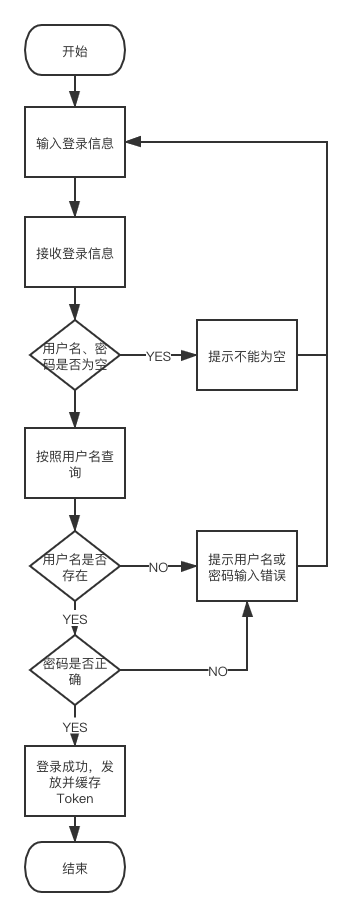
\includegraphics[width=0.4\textwidth,keepaspectratio]{data/chapter-5/login.png}
\caption{登录模块流程图}
\label{figure:login}
\end{figure}
\subsection{学生考试/练习模块}
该模块中列出了学生可以参加的所有练习和考试。学生选择其中一个考试/练习之后,系统开始计时,在考试过程中随机拍照并上传图片服务器,倒计时结束后自动交卷,
考生也可以在考试时间结束之前自行交卷。学生考试/练习模块流程图如\ref{figure:exam}所示。
\begin{figure}[H]
\centering
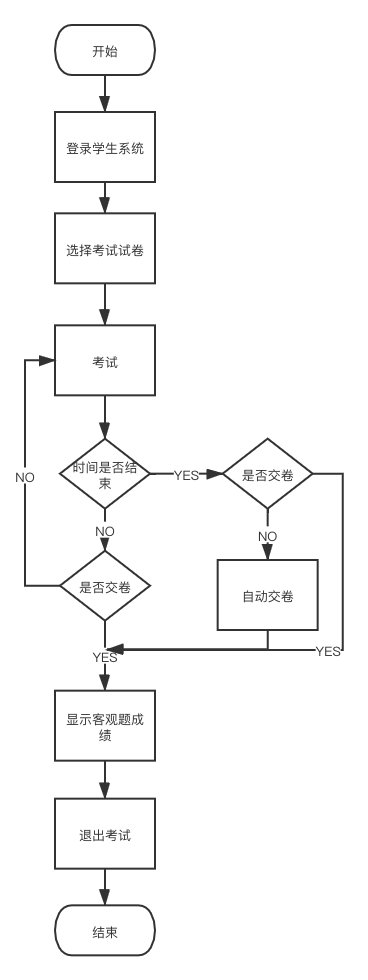
\includegraphics[width=0.5\textwidth,keepaspectratio]{data/chapter-5/exam.png}
\caption{考试模块流程图}
\label{figure:exam}
\end{figure}
\subsection{考试管理模块}
该模块主要用于添加、修改、删除考试信息。该模块结构图如图\ref{figure:examManage}所示。
\begin{figure}[H]
\centering
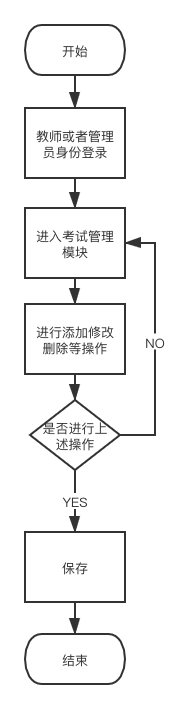
\includegraphics[width=0.3\textwidth,keepaspectratio]{data/chapter-5/examManage.png}
\caption{考试管理模块流程图}
\label{figure:examManage}
\end{figure}
\subsection{试题管理模块}
该模块主要用于试题库的建设和维护,可以对试题进行添加、删除、修改和查询。该模块结构图如图\ref{figure:question}所示。
\begin{figure}[H]
\centering
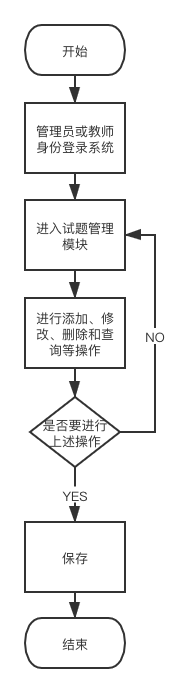
\includegraphics[width=0.3\textwidth,keepaspectratio]{data/chapter-5/question.png}
\caption{试题管理模块流程图}
\label{figure:question}
\end{figure}
\subsection{组卷管理模块}
该模块主要用于提供试卷。可以有教师手工组卷,具体操作如下:进入手工组卷页面,选择相关的科目即可从题库中调出相关题目的列表。
该模块结构图如图\ref{figure:makeup}所示。
\begin{figure}[H]
\centering
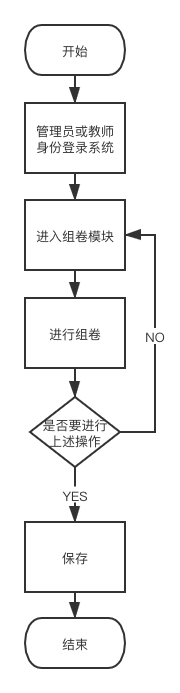
\includegraphics[width=0.2\textwidth,keepaspectratio]{data/chapter-5/makeup.png}
\caption{组卷模块流程图}
\label{figure:makeup}
\end{figure}
\subsection{成绩管理模块}
该模块主要用于查看学生考试的历史记录以及对为批改的主观题进行评分和评语。
\subsection{个人信息管理模块}
该模块主要用于用户对自己信息进行修改。该模块结构图如图\ref{figure:information}所示。
\begin{figure}[H]
\centering
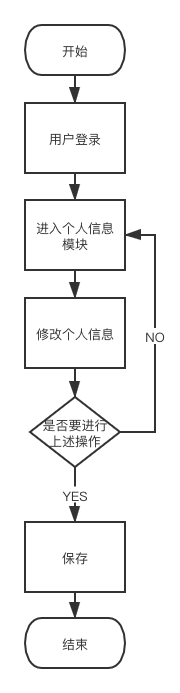
\includegraphics[width=0.3\textwidth,keepaspectratio]{data/chapter-5/information.png}
\caption{个人信息管理模块}
\label{figure:information}
\end{figure}

\section{管理员子系统的具体实现}
\subsection{登录}
\begin{enumerate}
	\item[] \textbf{功能描述:}通过管理员的用户名和密码进行登录。
	\item[] \textbf{功能页面:}如图\ref{figure:denglu}所示 \\
		\begin{figure}[H]
			\centering
			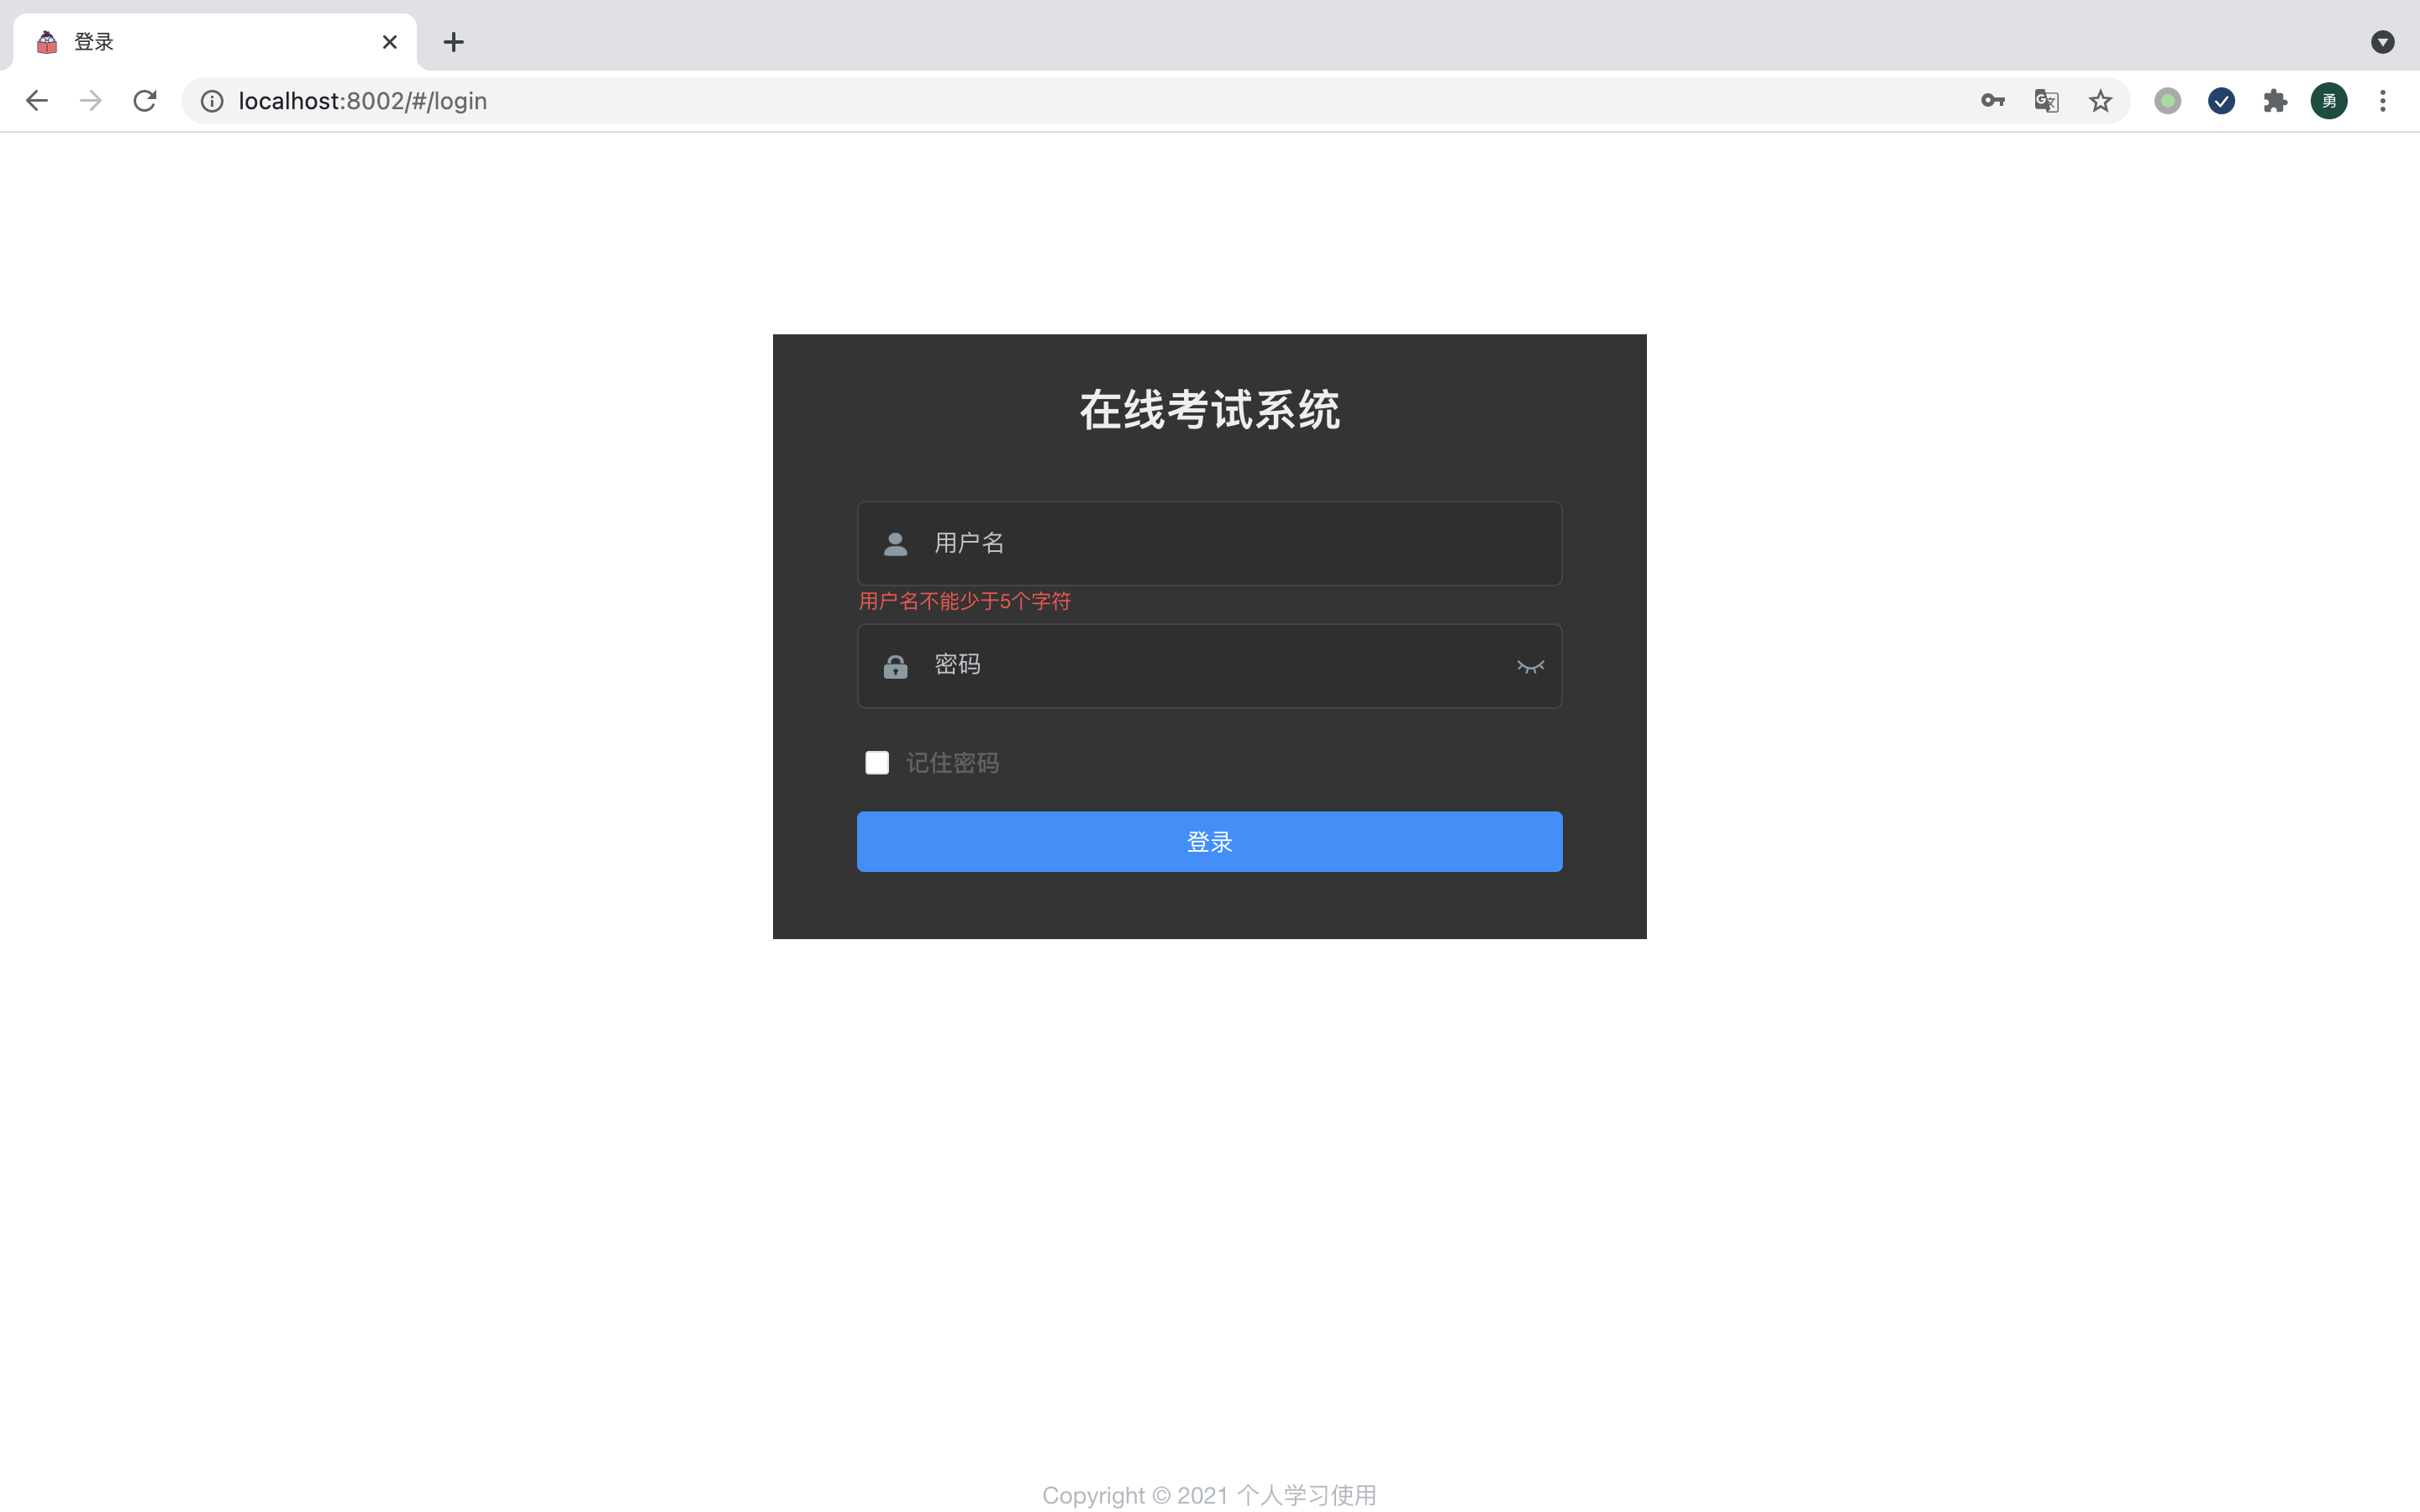
\includegraphics[width=1.0\textwidth,keepaspectratio]{data/chapter-5/denglu.png}
			\caption{登录页面}
			\label{figure:denglu}
		\end{figure}
\end{enumerate}

\subsection{主页}
\begin{enumerate}
	\item[] \textbf{功能描述:}管理员界面的仪表盘,显示常用数据。
	\item[] \textbf{功能页面:}如图\ref{figure:zhuye}所示 \\
		\begin{figure}[H]
			\centering
			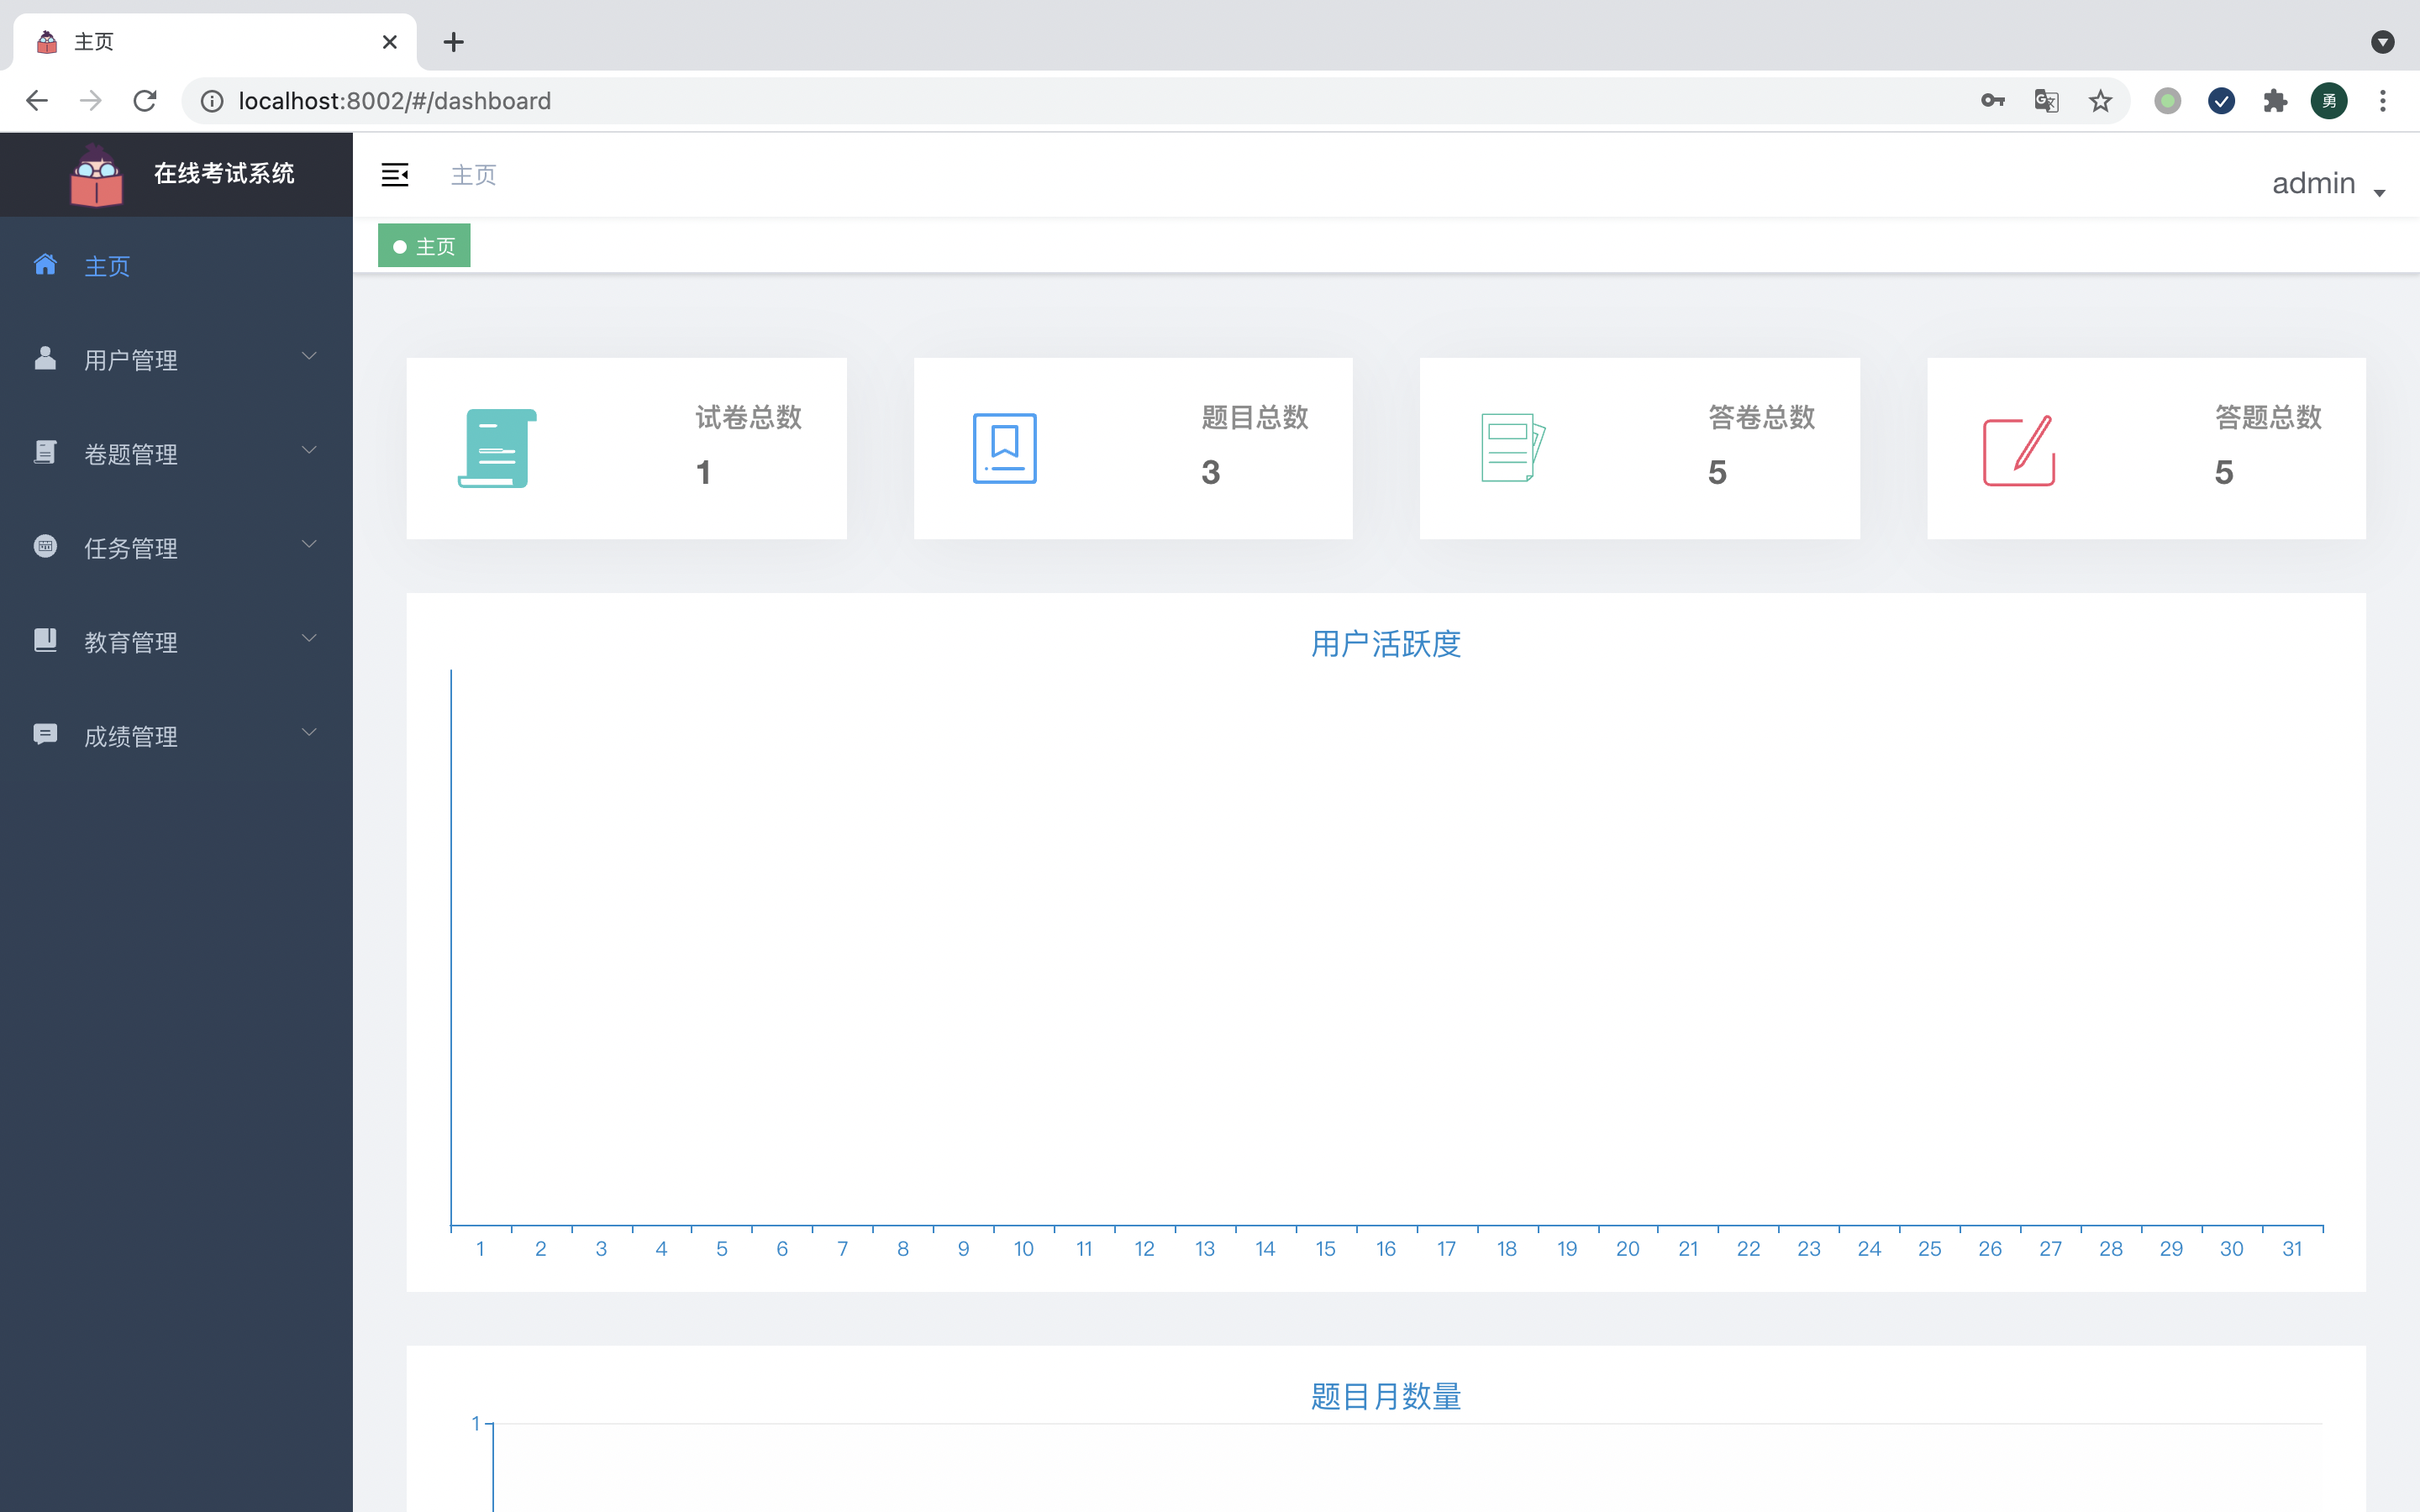
\includegraphics[width=1.0\textwidth,keepaspectratio]{data/chapter-5/zhuye.png}
			\caption{管理员主页}
			\label{figure:zhuye}
		\end{figure}
\end{enumerate}

\subsection{用户管理}
\begin{enumerate}
	\item[] \textbf{功能描述:}用户管理功能界面,可以对所有用户进行信息的修改,同时可以添加或删除用户。
	\item[] \textbf{功能页面:}如图\ref{figure:yonghu}所示 \\
		\begin{figure}[H]
			\centering
			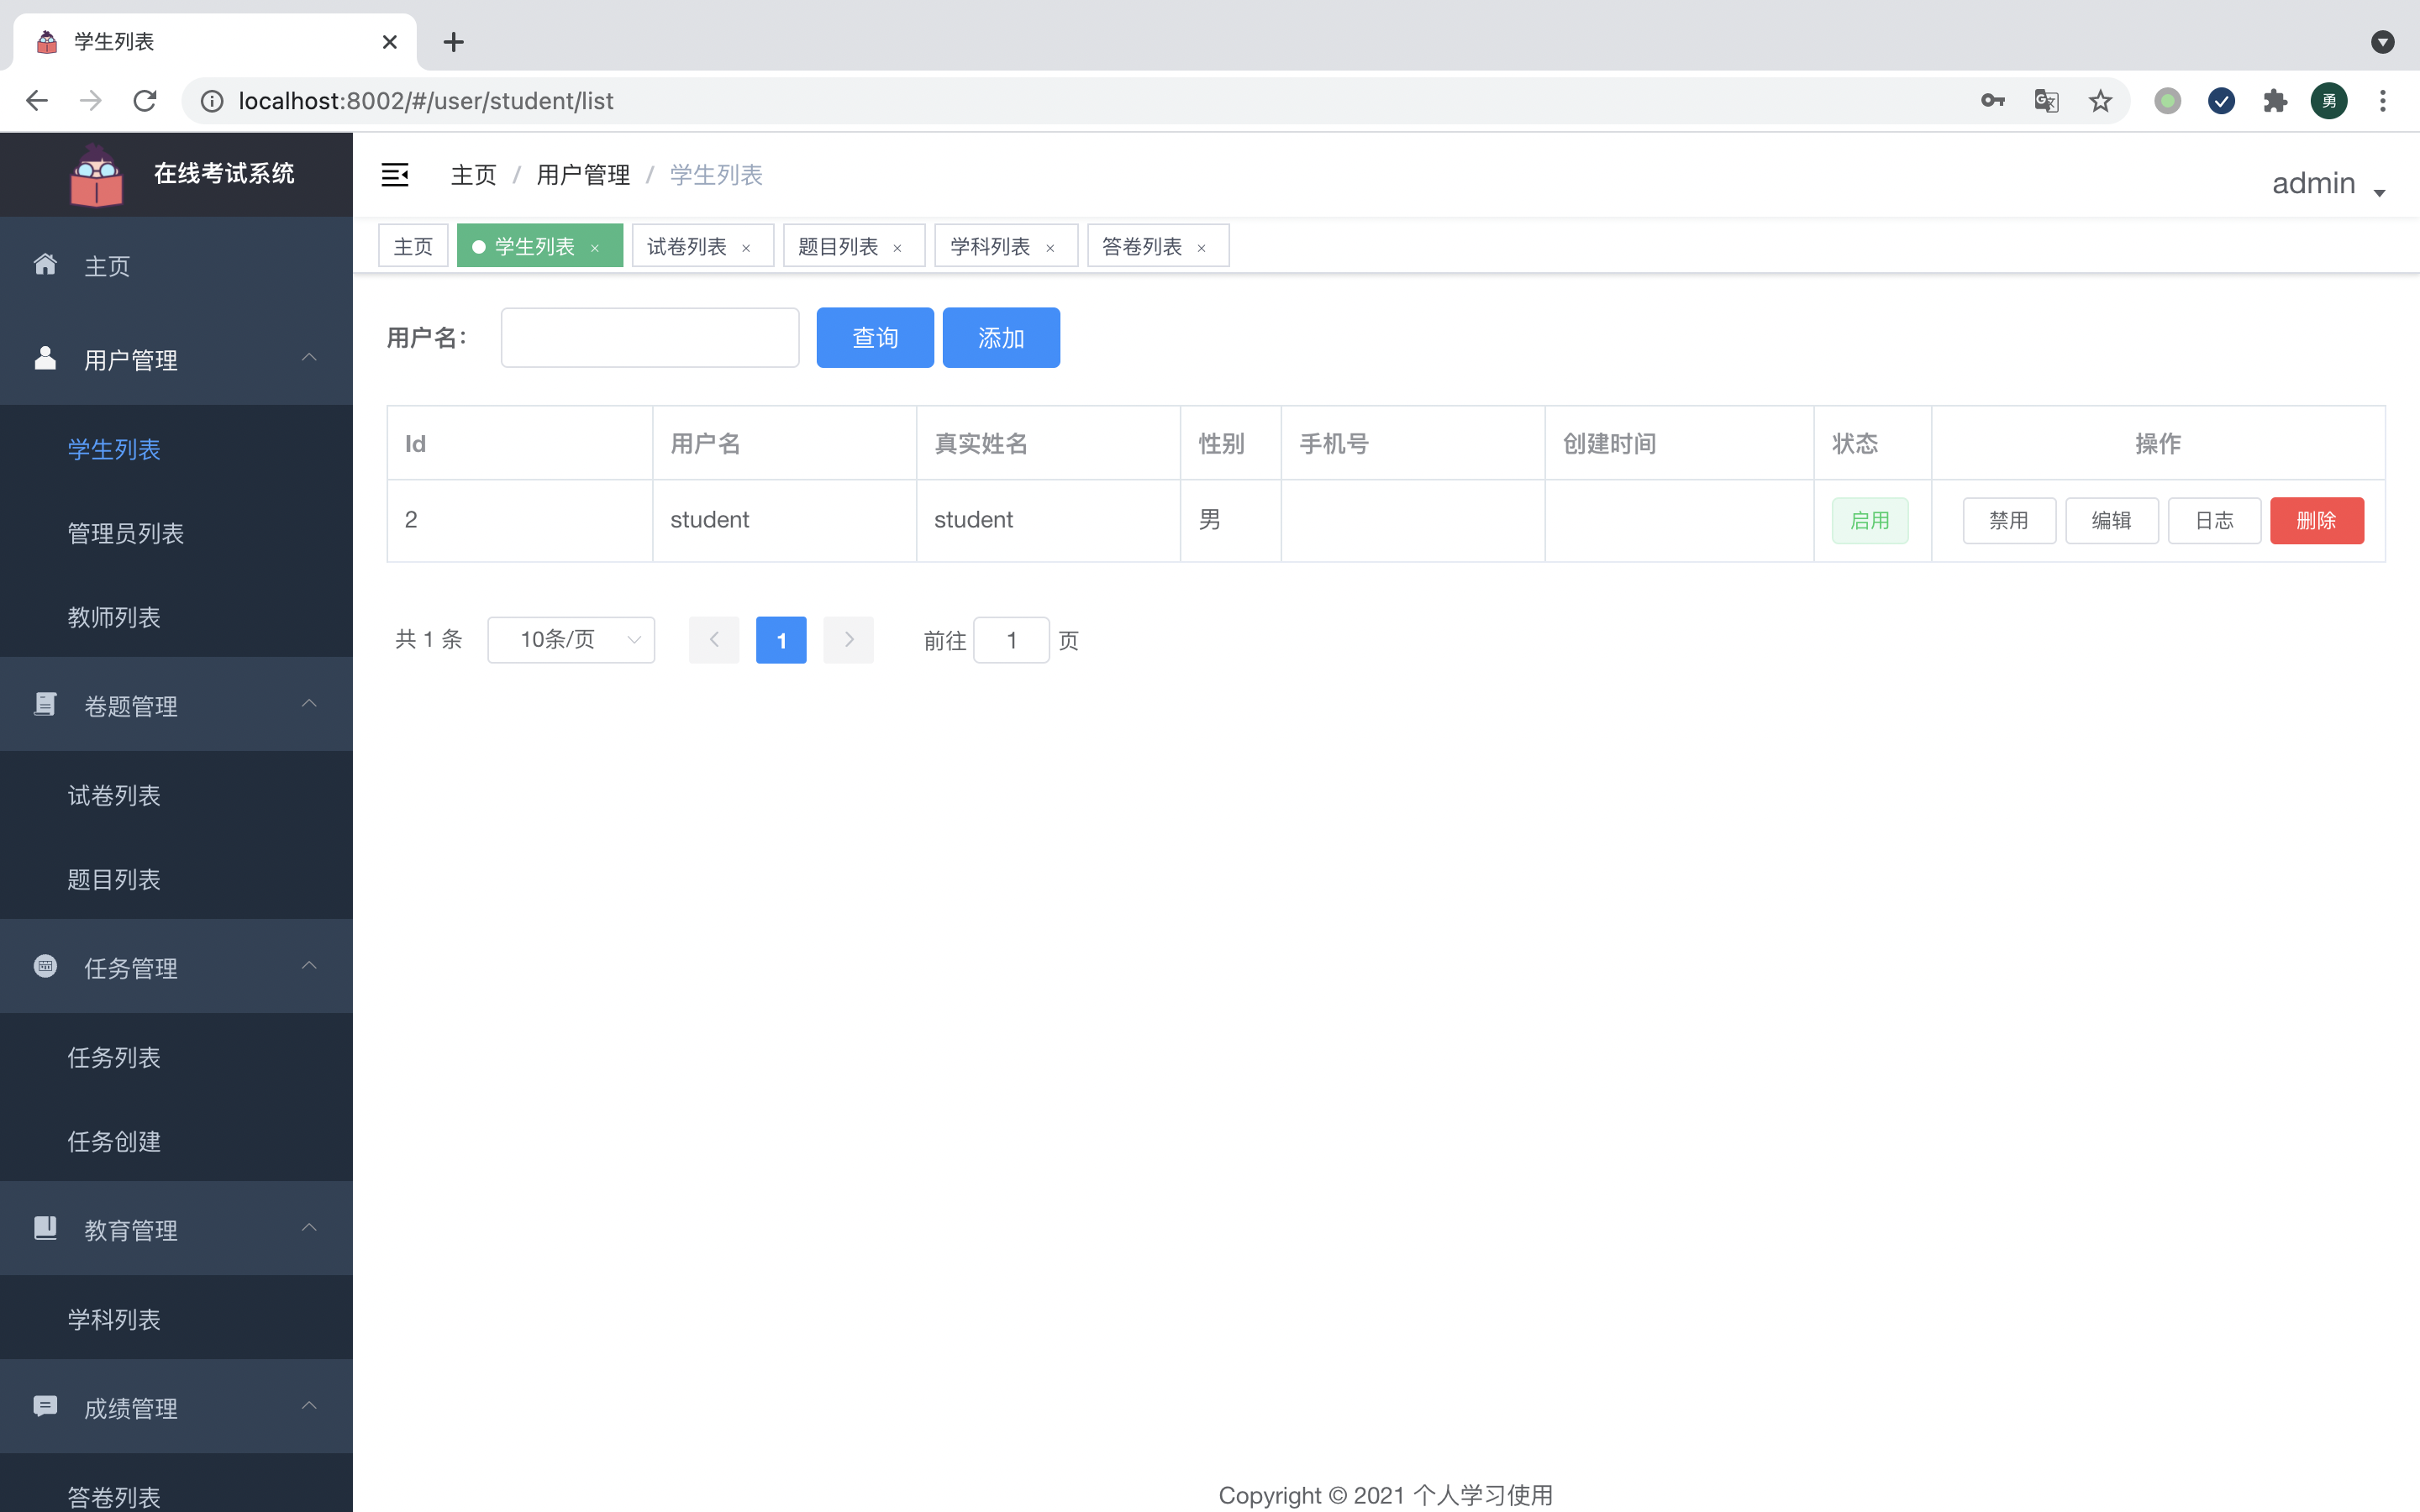
\includegraphics[width=1.0\textwidth,keepaspectratio]{data/chapter-5/yonghu.png}
			\caption{用户管理}
			\label{figure:yonghu}
		\end{figure}
\end{enumerate}

\subsection{试卷管理}
\begin{enumerate}
	\item[] \textbf{功能描述:}试卷管理功能界面,可以对所有试卷进行内容的修改,同时可以添加或删除试卷。
	\item[] \textbf{功能页面:}如图\ref{figure:shijuan}所示 \\
		\begin{figure}[H]
			\centering
			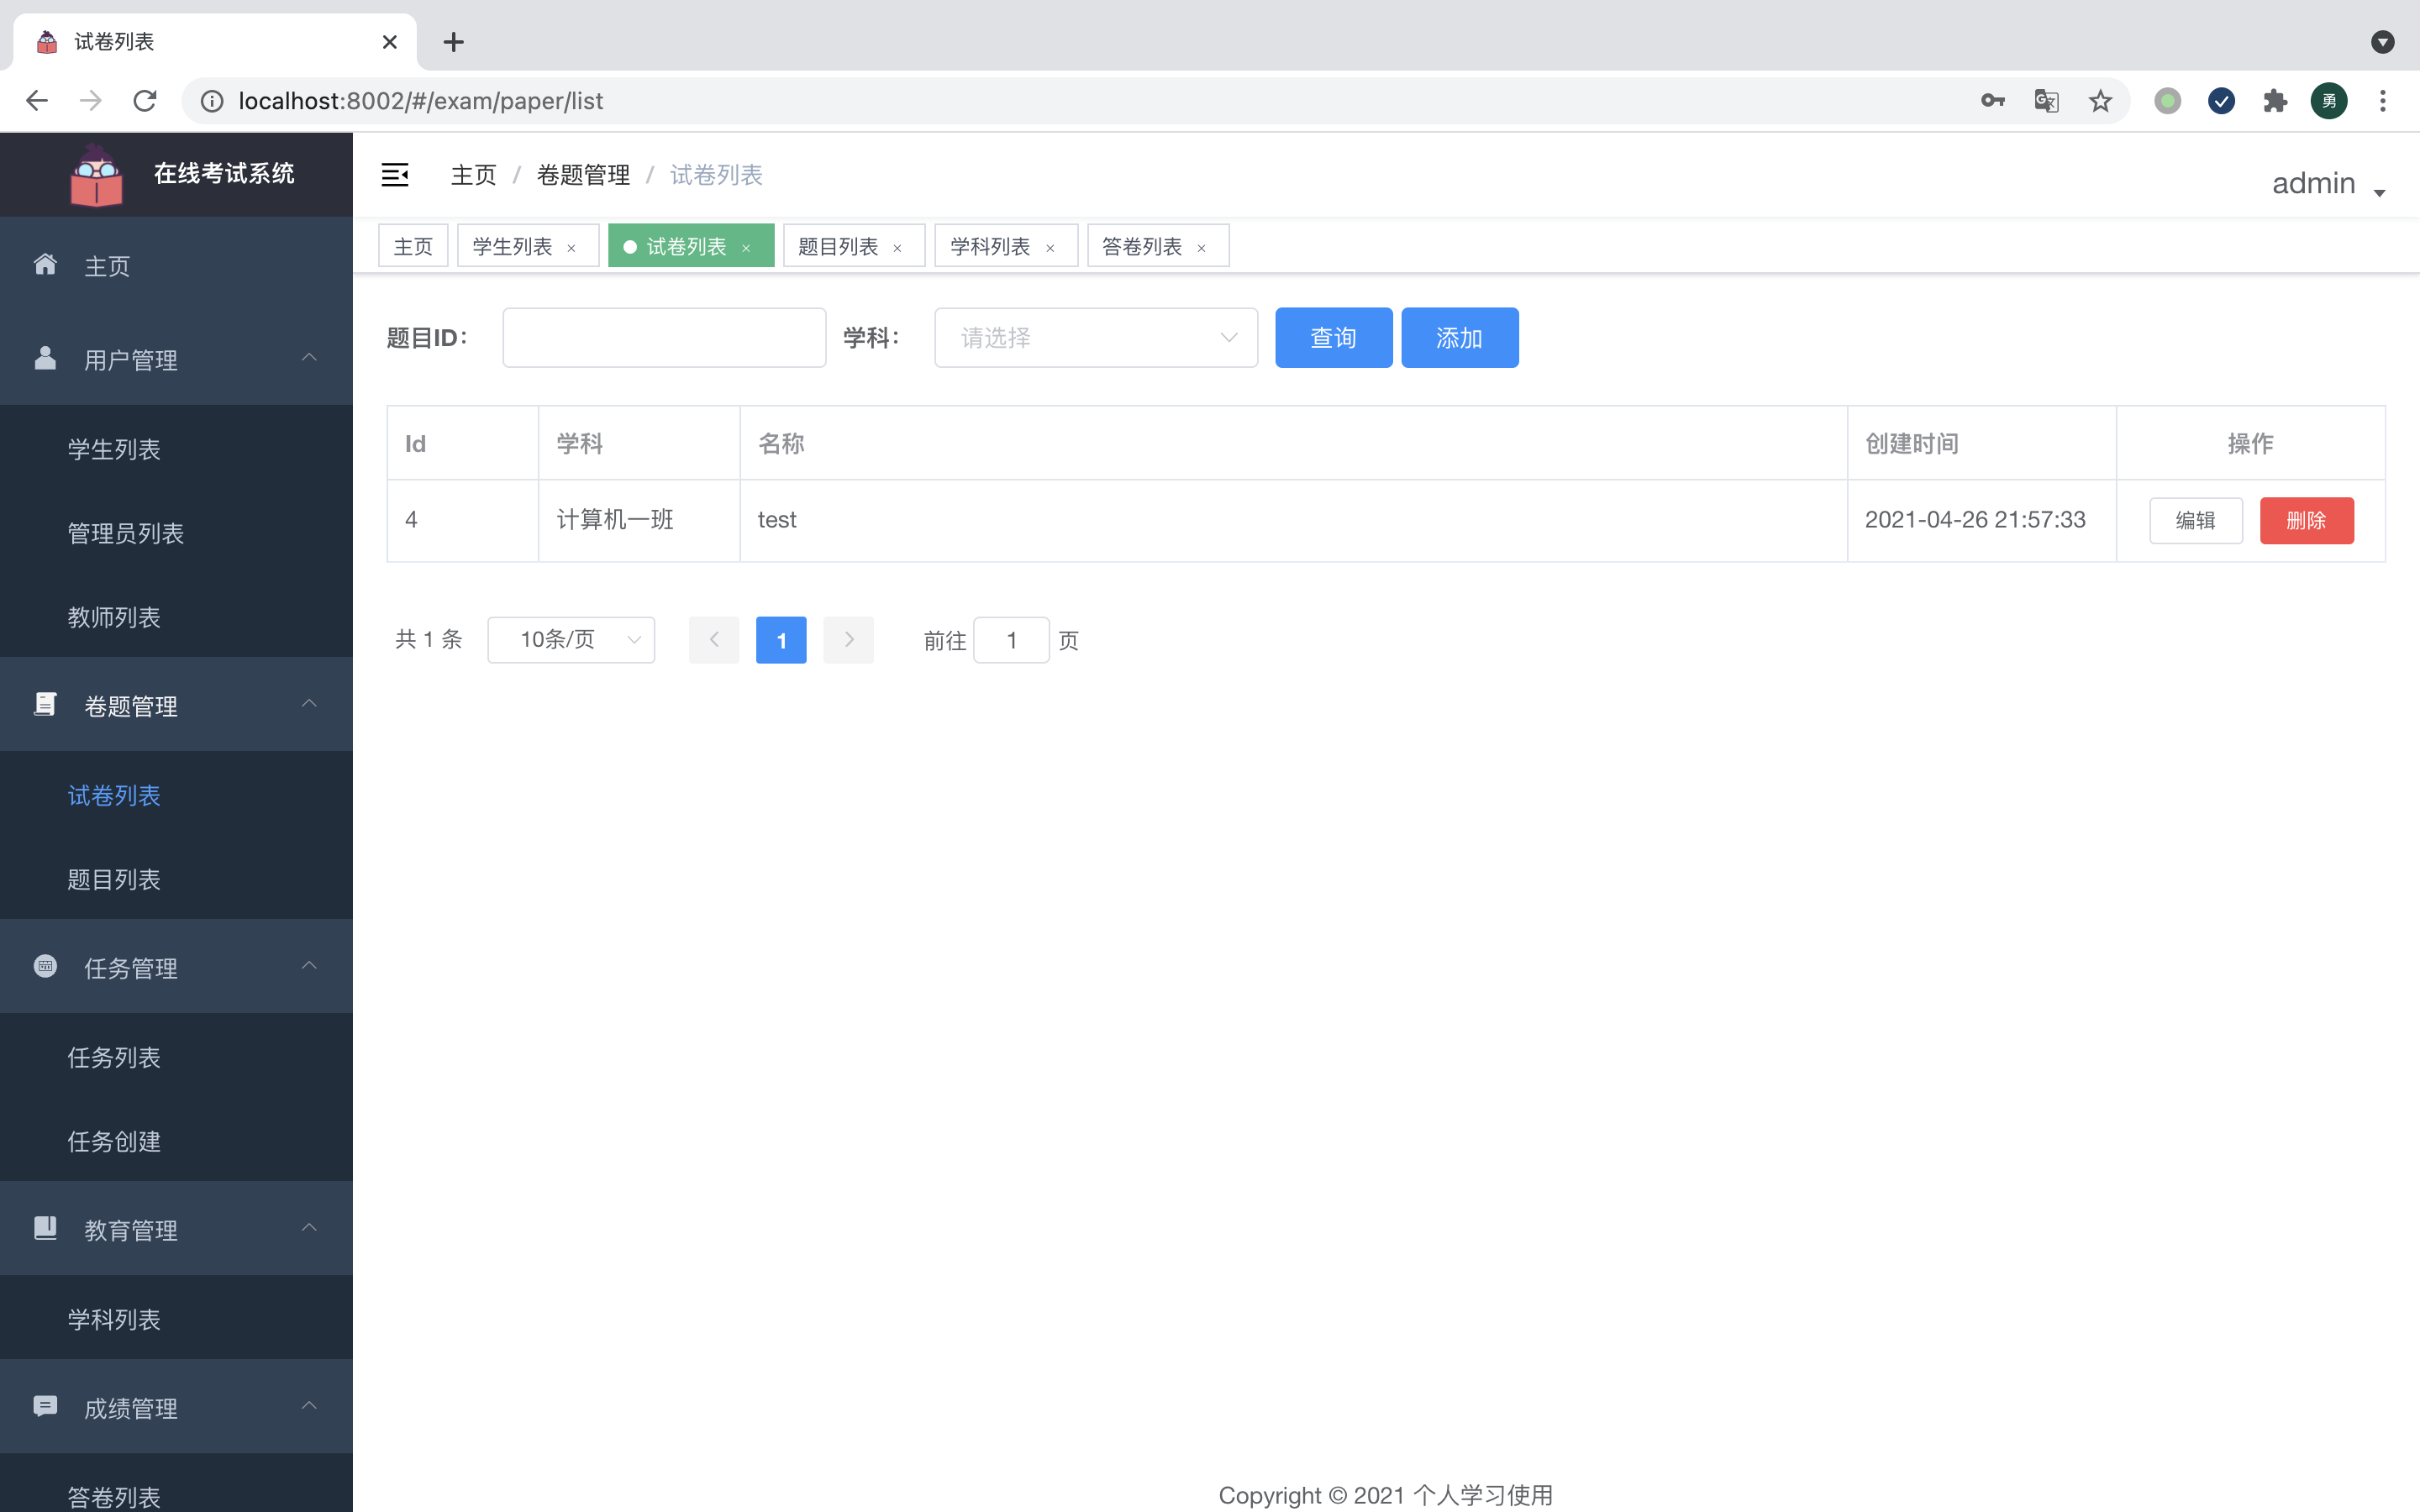
\includegraphics[width=1.0\textwidth,keepaspectratio]{data/chapter-5/shijuan.png}
			\caption{试卷管理}
			\label{figure:shijuan}
		\end{figure}
\end{enumerate}

\subsection{试题管理}
\begin{enumerate}
	\item[] \textbf{功能描述:}试题管理功能界面,可以对所有试题进行内容的修改,同时可以添加或删除试题。
	\item[] \textbf{功能页面:}如图\ref{figure:timu}所示 \\
		\begin{figure}[H]
			\centering
			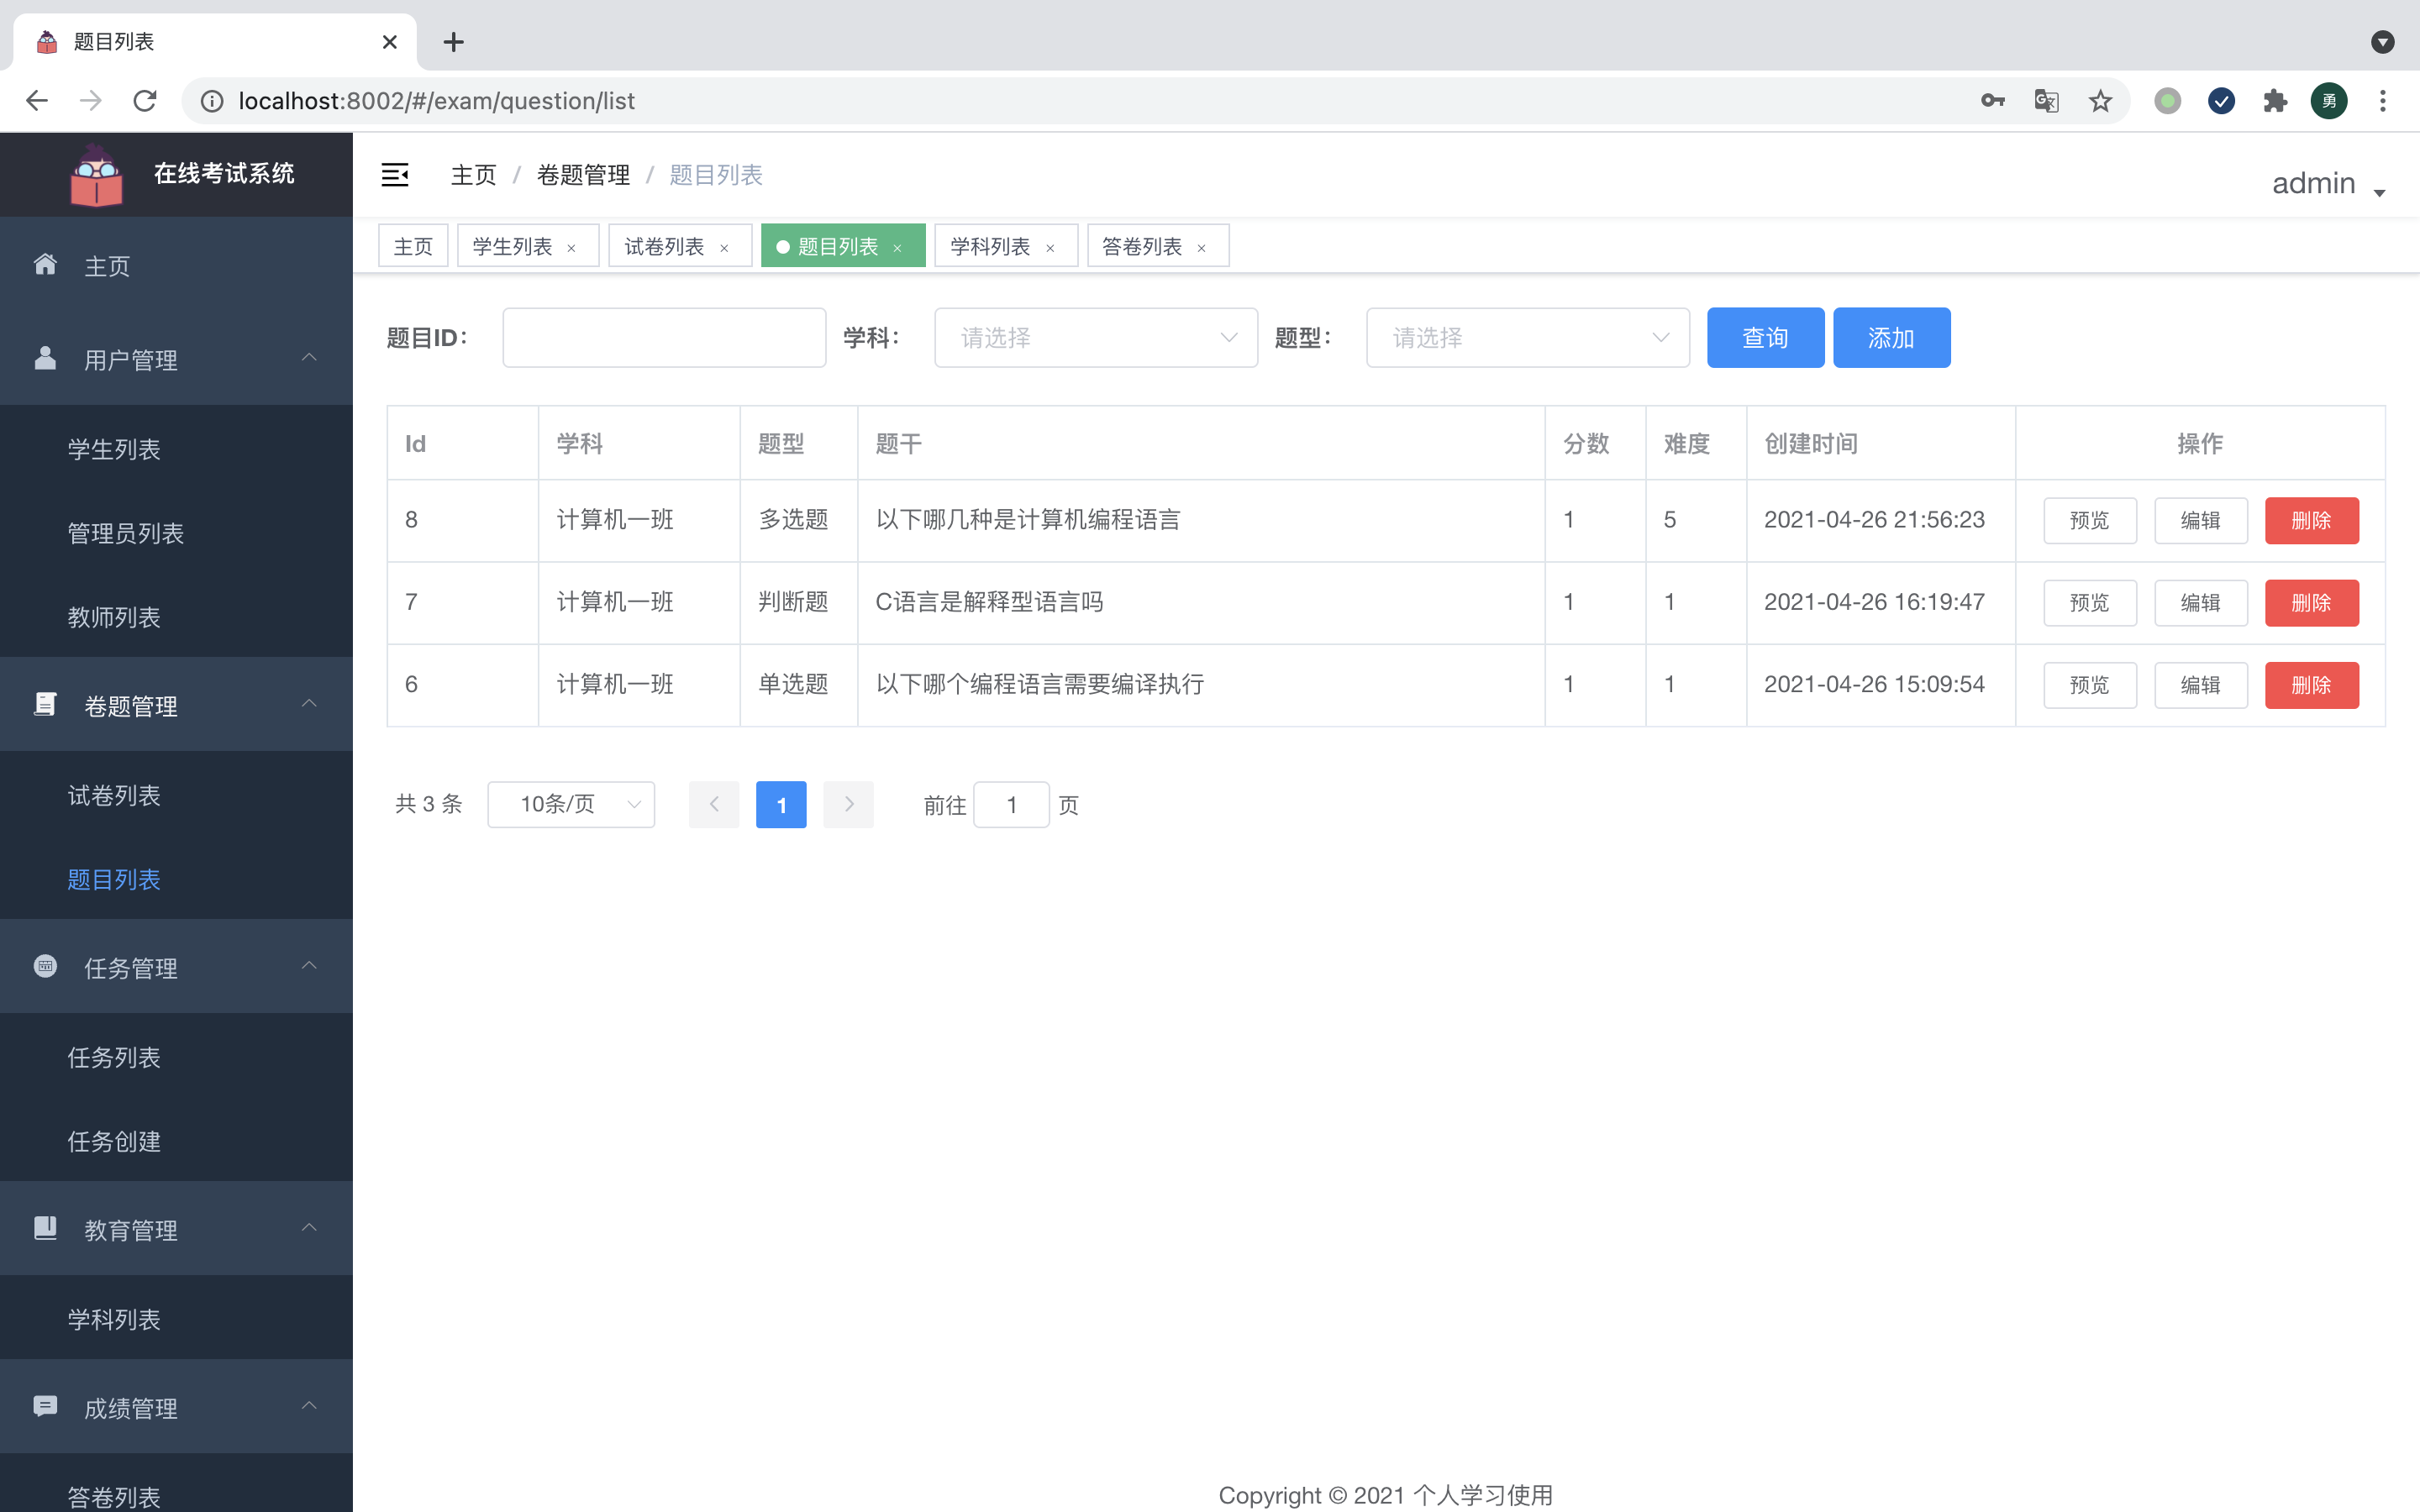
\includegraphics[width=1.0\textwidth,keepaspectratio]{data/chapter-5/timu.png}
			\caption{试题管理}
			\label{figure:timu}
		\end{figure}
\end{enumerate}

\subsection{班级管理}
\begin{enumerate}
	\item[] \textbf{功能描述:}班级管理功能界面,可以对所有班级进行信息的修改,同时可以添加或删除班级。
	\item[] \textbf{功能页面:}如图\ref{figure:xueke}所示 \\
		\begin{figure}[H]
			\centering
			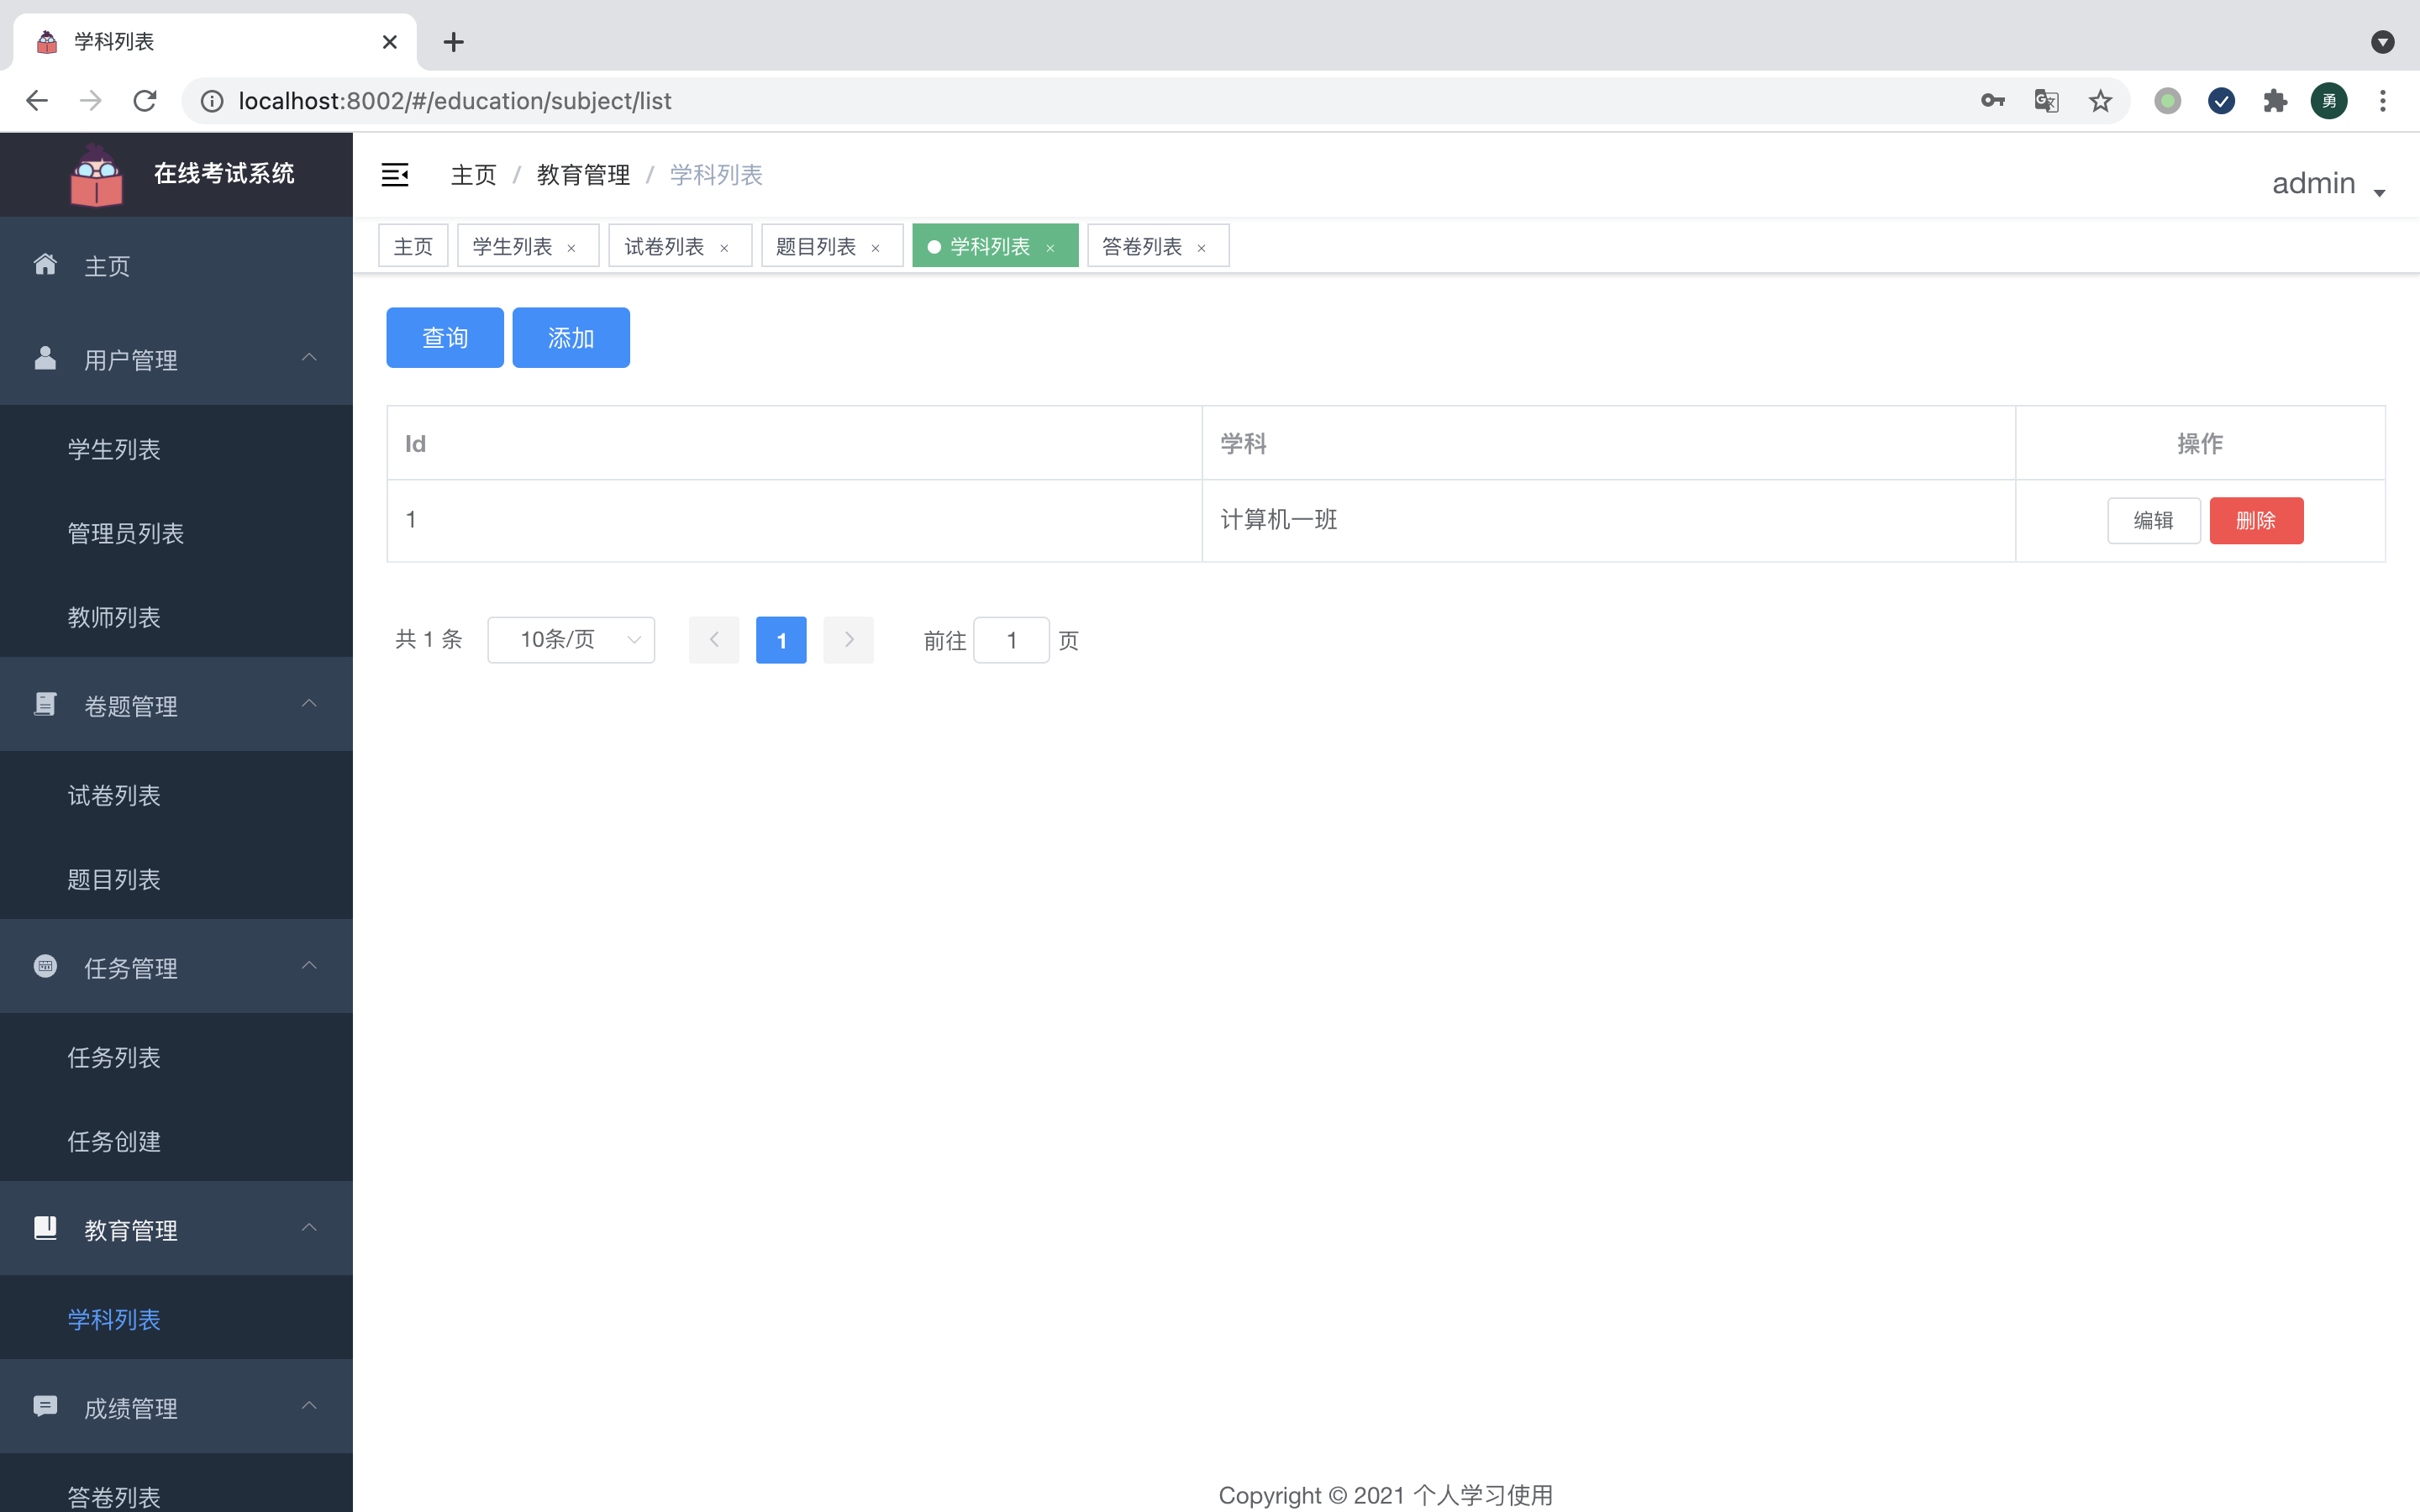
\includegraphics[width=1.0\textwidth,keepaspectratio]{data/chapter-5/xueke.png}
			\caption{班级管理}
			\label{figure:xueke}
		\end{figure}
\end{enumerate}

\subsection{教育管理}
\begin{enumerate}
	\item[] \textbf{功能描述:}教育管理功能界面,试卷的批改和历史试卷的查看。
	\item[] \textbf{功能页面:}如图\ref{figure:dajuan}所示 \\
		\begin{figure}[H]
			\centering
			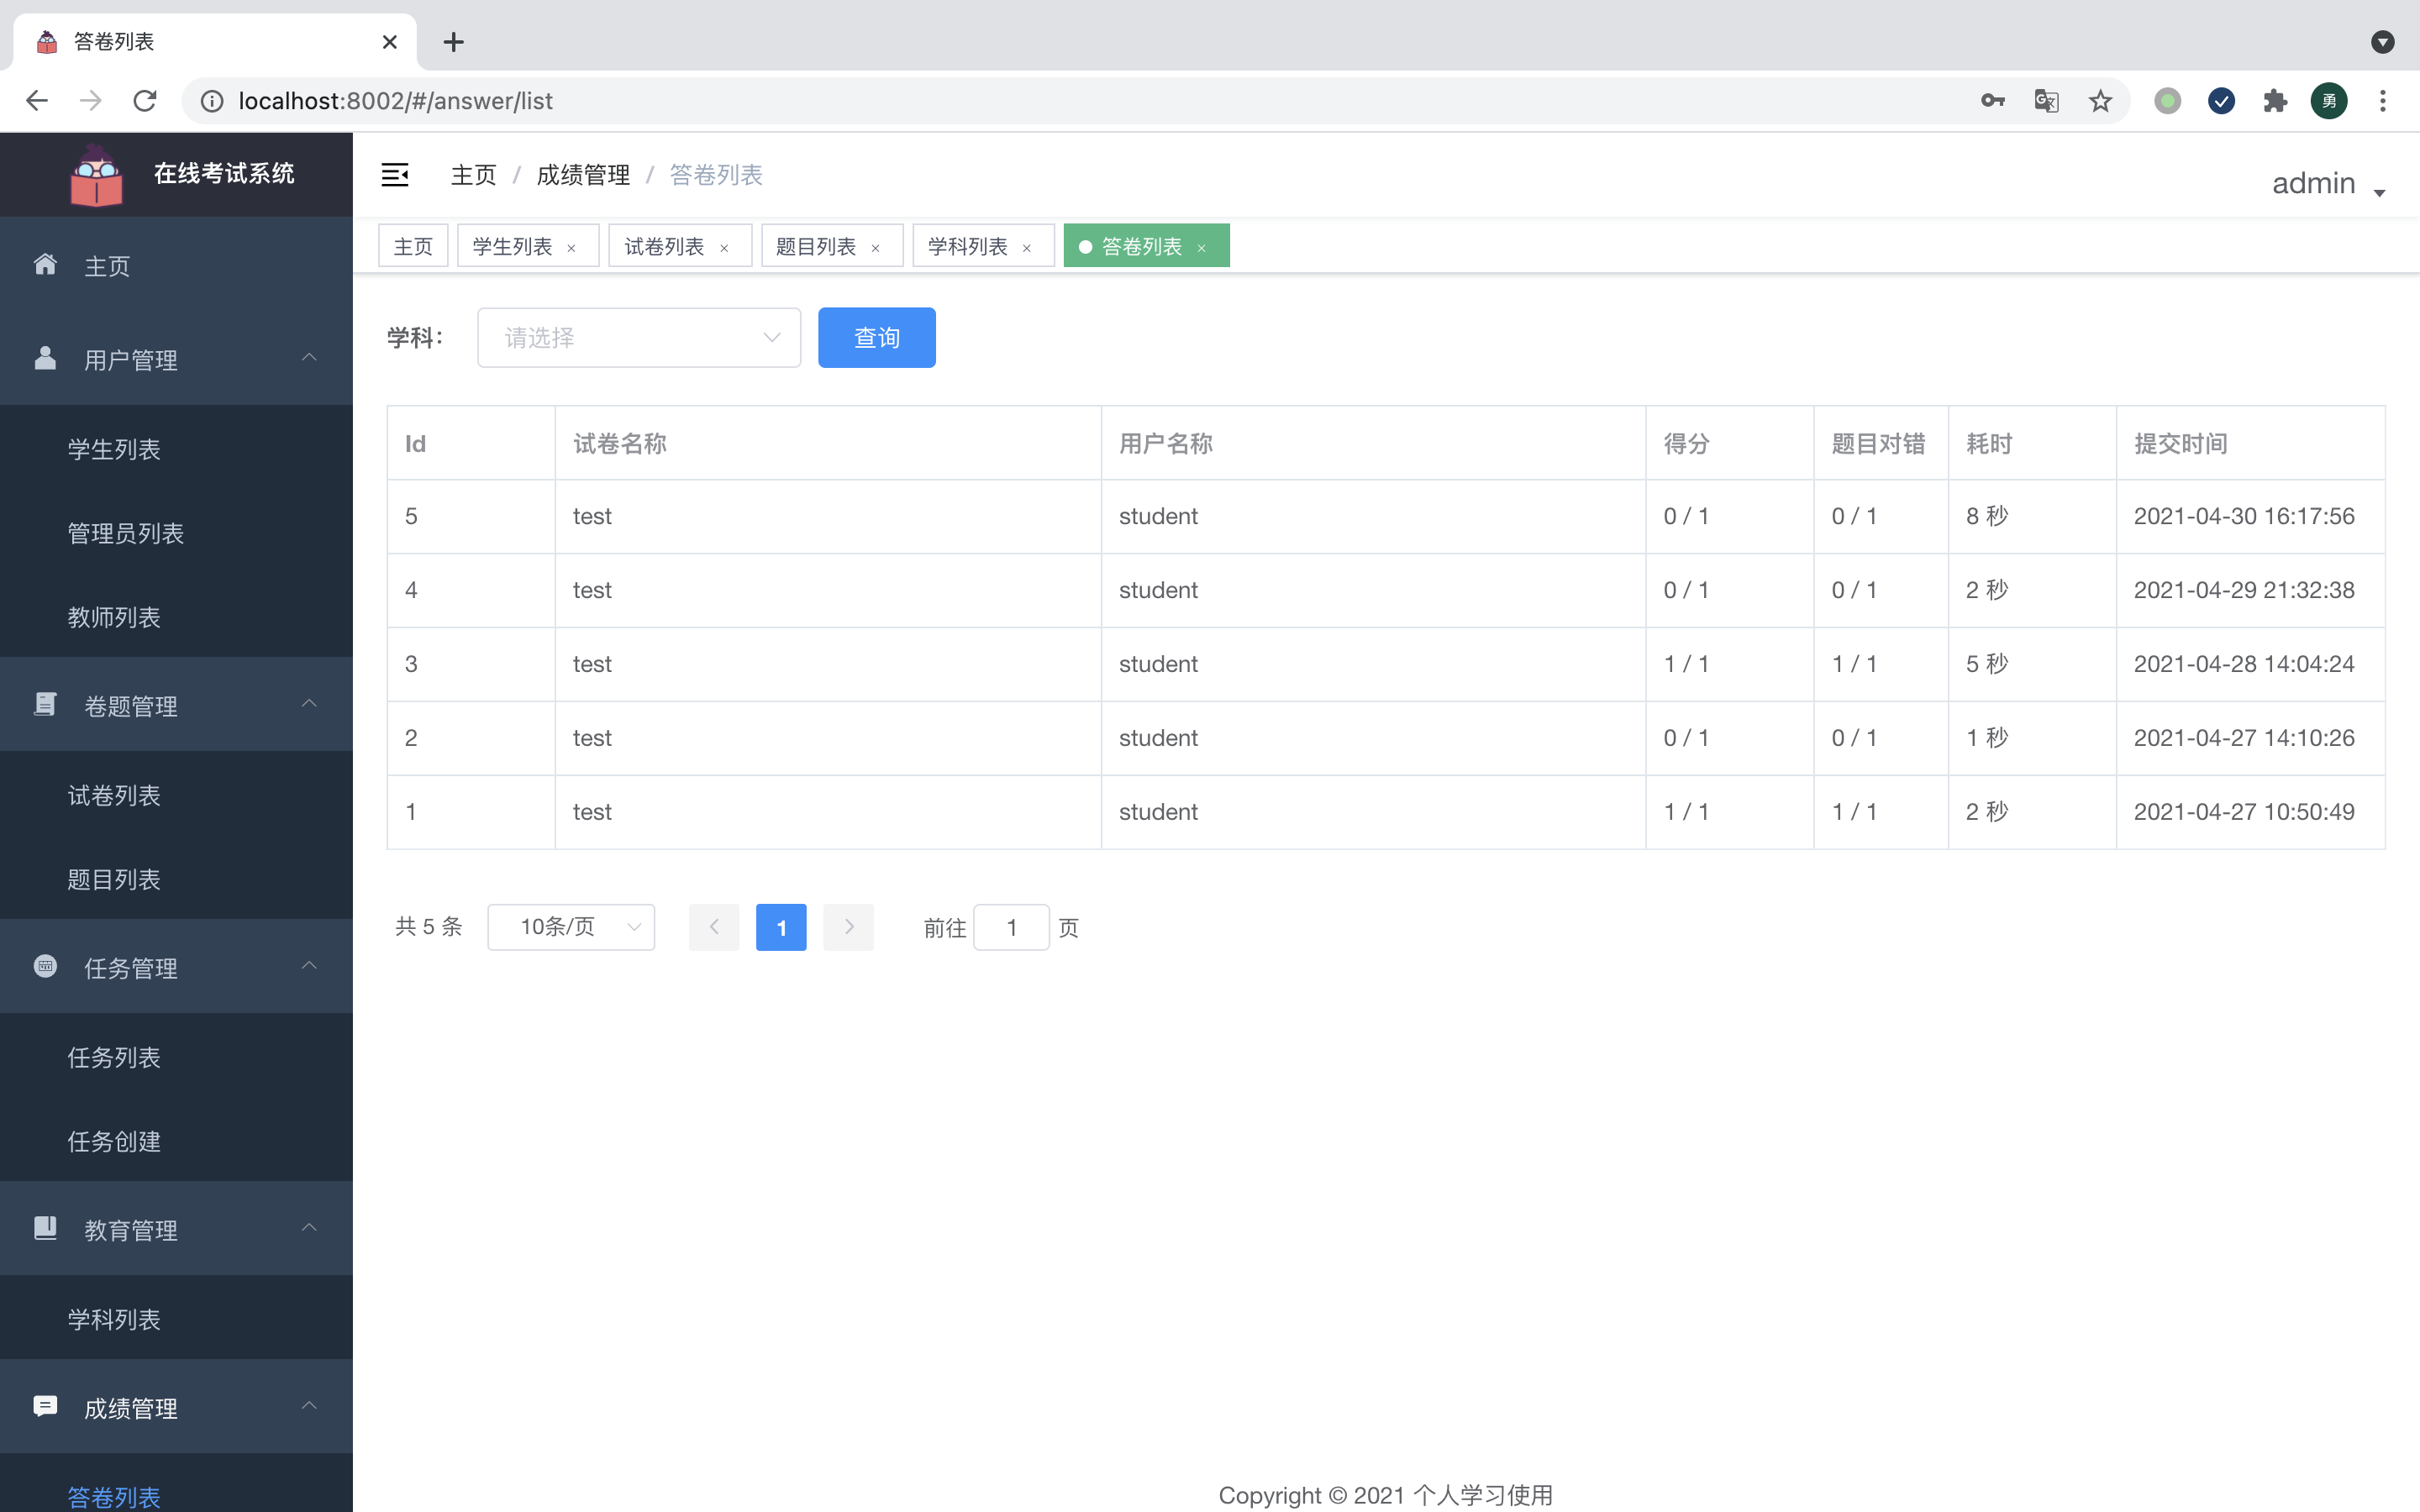
\includegraphics[width=1.0\textwidth,keepaspectratio]{data/chapter-5/dajuan.png}
			\caption{教育管理}
			\label{figure:dajuan}
		\end{figure}
\end{enumerate}

\section{老师子系统的具体实现}
老师子系统和管理员子系统的页面和逻辑大致相同,区别在于老师管理的对象为学生而不是全部用户,这里就不一一列出了。

\section{学生子系统的具体实现}
\subsection{学生登录}
\begin{enumerate}
	\item[] \textbf{功能描述:}学生登录界面,学生通过用户名和密码进行登录。
	\item[] \textbf{功能页面:}如图\ref{figure:sdenglu}所示 \\
		\begin{figure}[H]
			\centering
			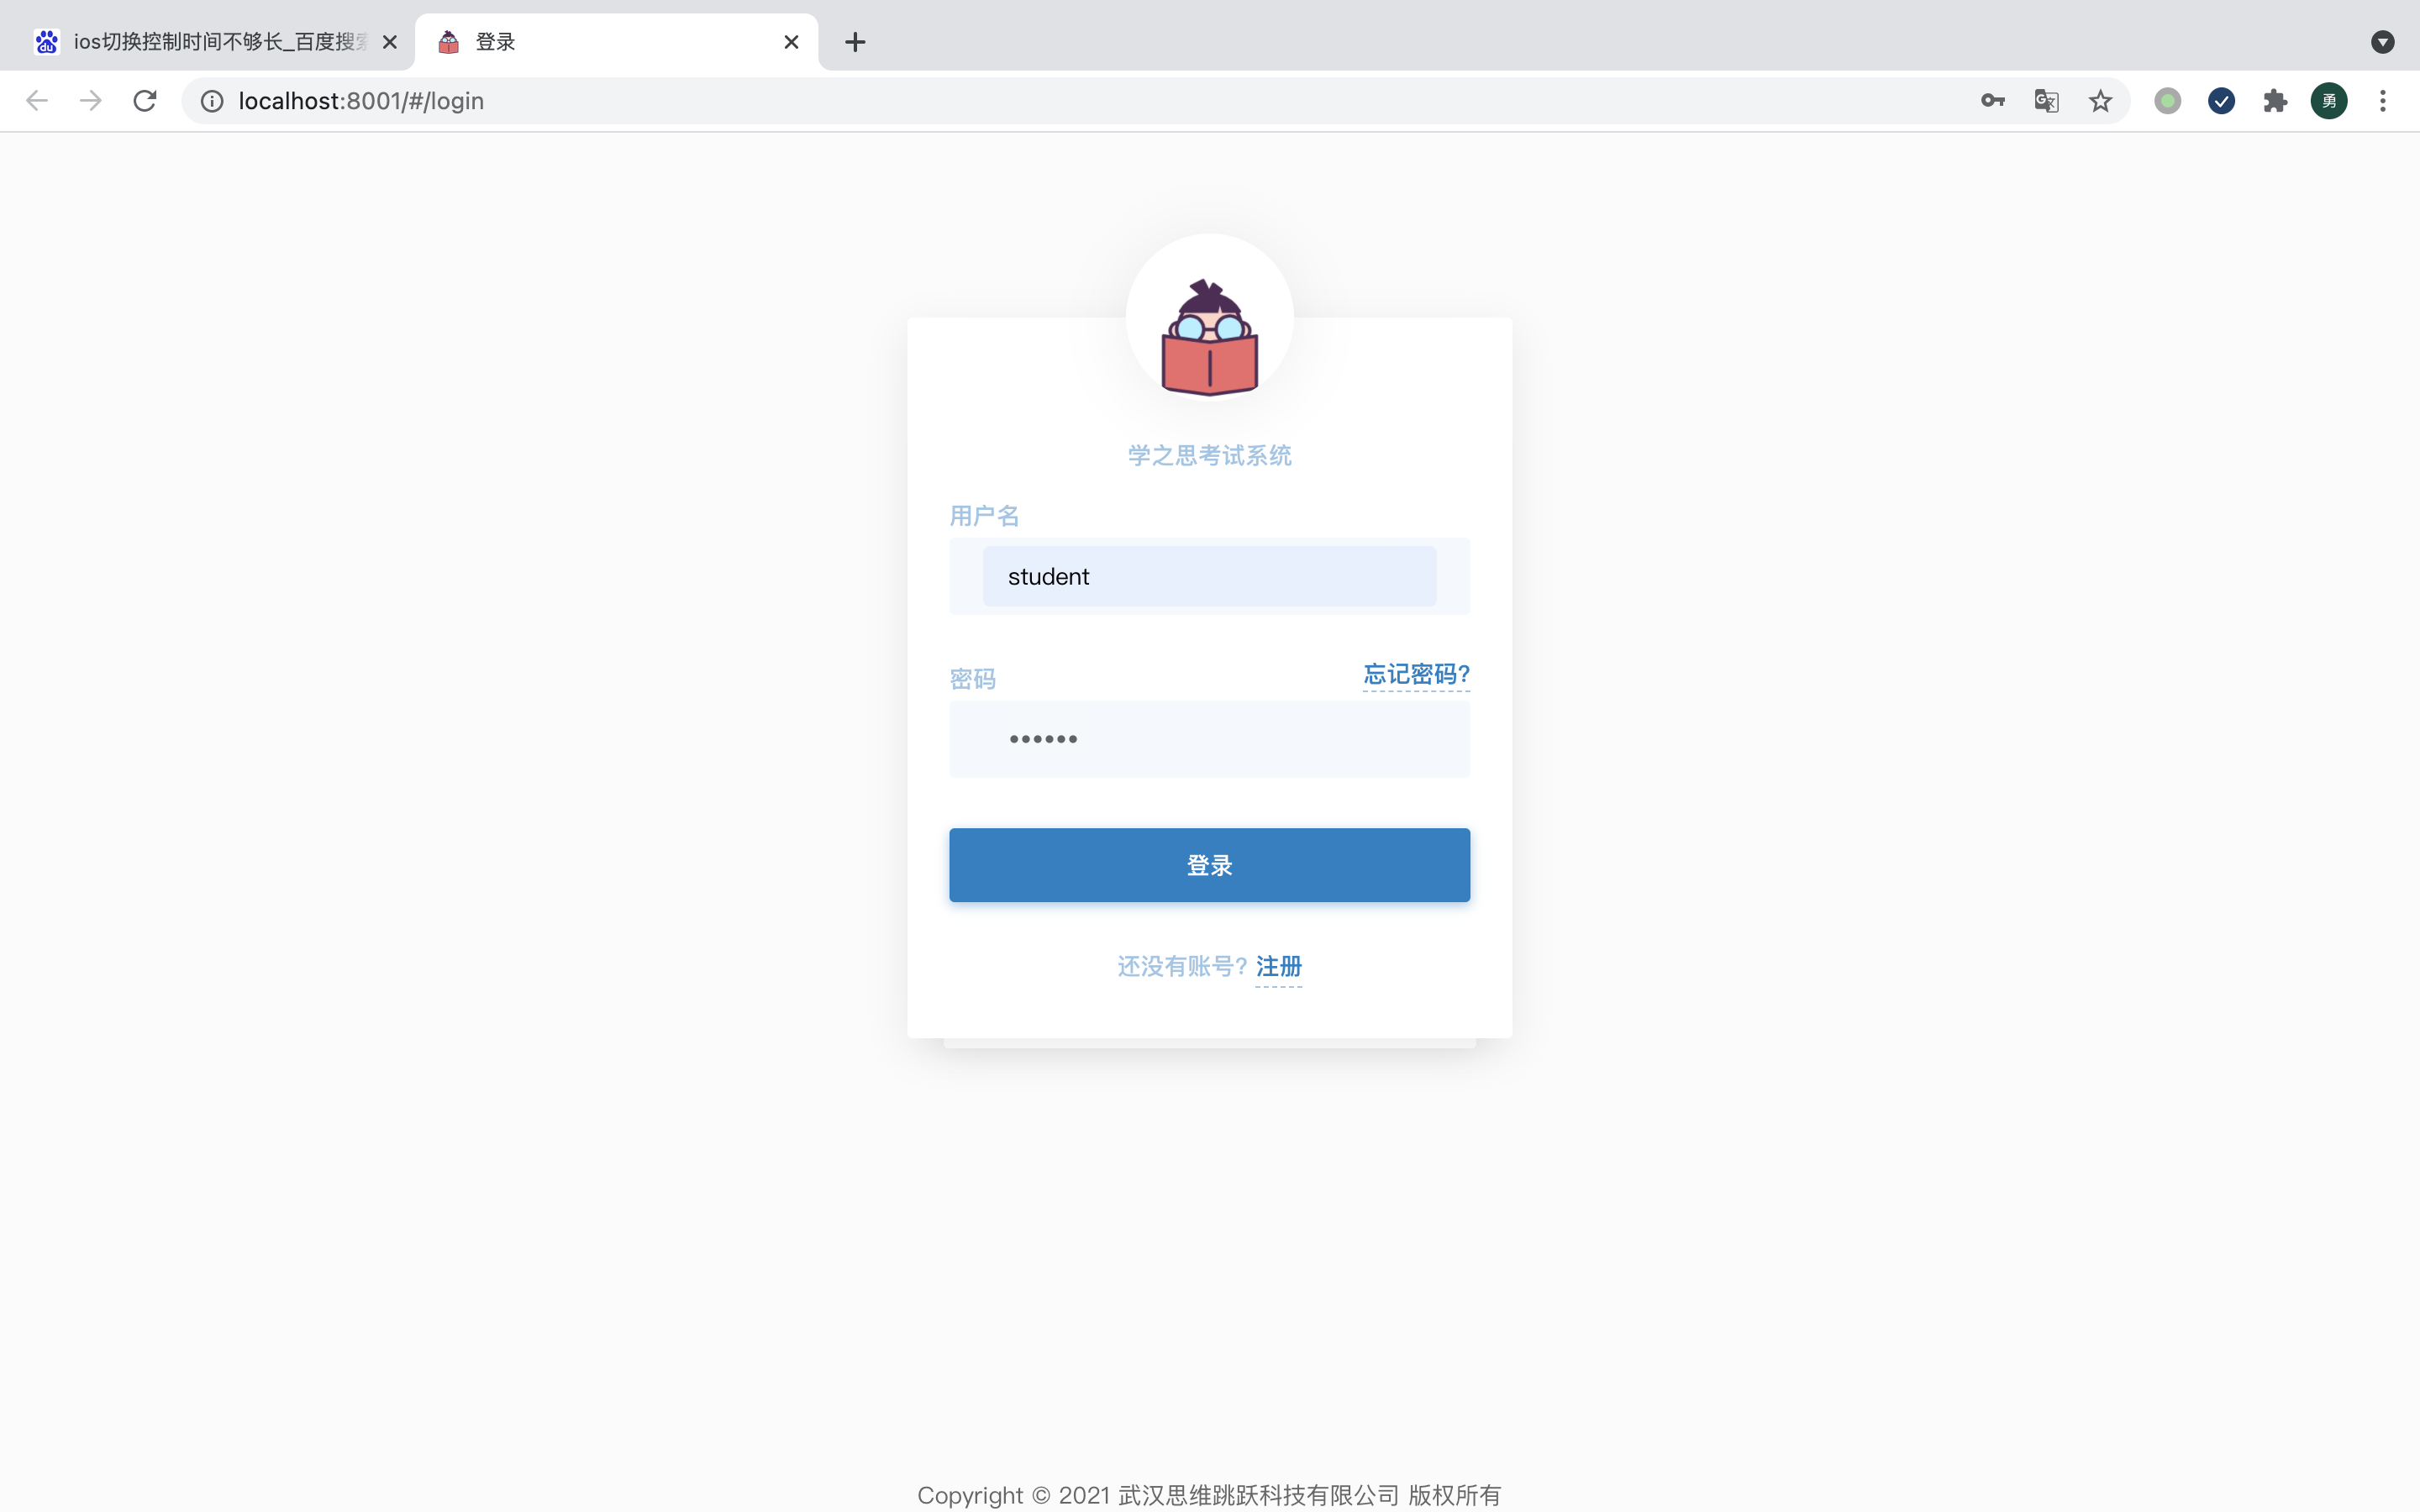
\includegraphics[width=1.0\textwidth,keepaspectratio]{data/chapter-5/student/denglu.png}
			\caption{学生登录}
			\label{figure:sdenglu}
		\end{figure}
\end{enumerate}

\subsection{学生主页}
\begin{enumerate}
	\item[] \textbf{功能描述:}学生系统的主页界面,展示一些主要信息,例如该学生可以进行的考试。
	\item[] \textbf{功能页面:}如图\ref{figure:szhuye}所示 \\
		\begin{figure}[H]
			\centering
			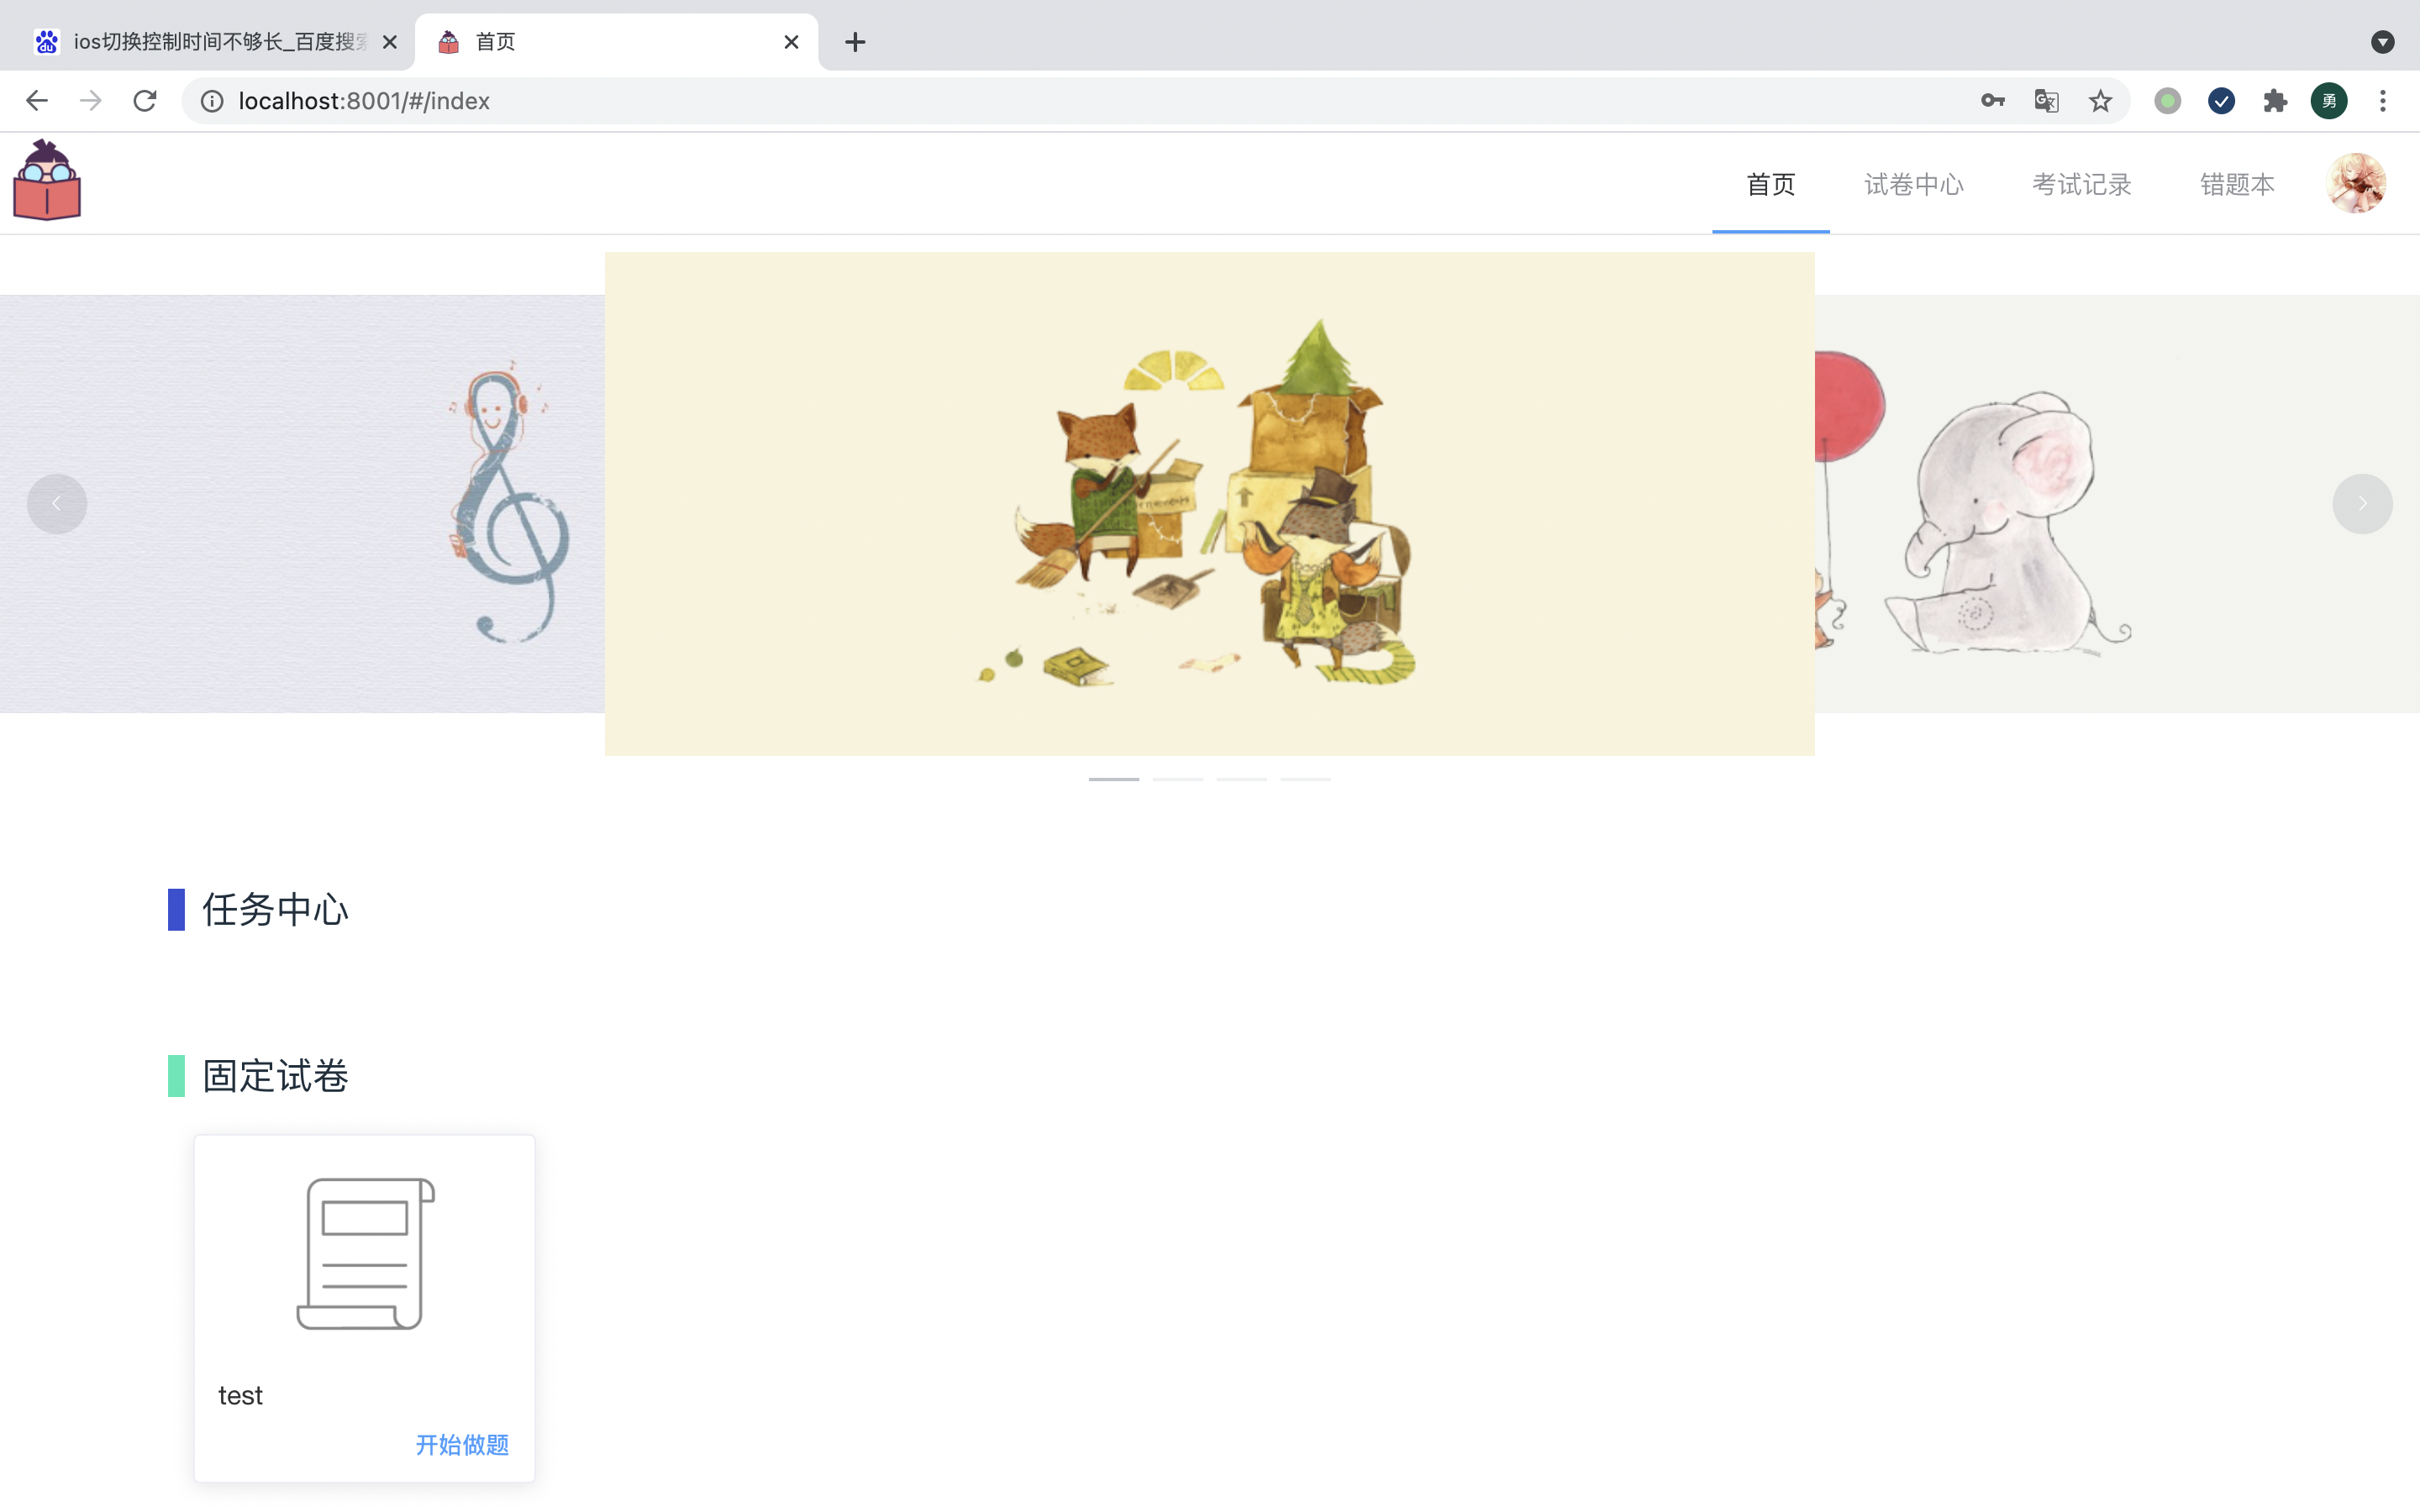
\includegraphics[width=1.0\textwidth,keepaspectratio]{data/chapter-5/student/zhuye.png}
			\caption{学生主页}
			\label{figure:szhuye}
		\end{figure}
\end{enumerate}

\subsection{学生试卷中心}
\begin{enumerate}
	\item[] \textbf{功能描述:}试卷中心功能界面,学生可以通过试卷中心找到所有公开的固定试卷和时段试卷。
	\item[] \textbf{功能页面:}如图\ref{figure:szhongxin}所示 \\
		\begin{figure}[H]
			\centering
			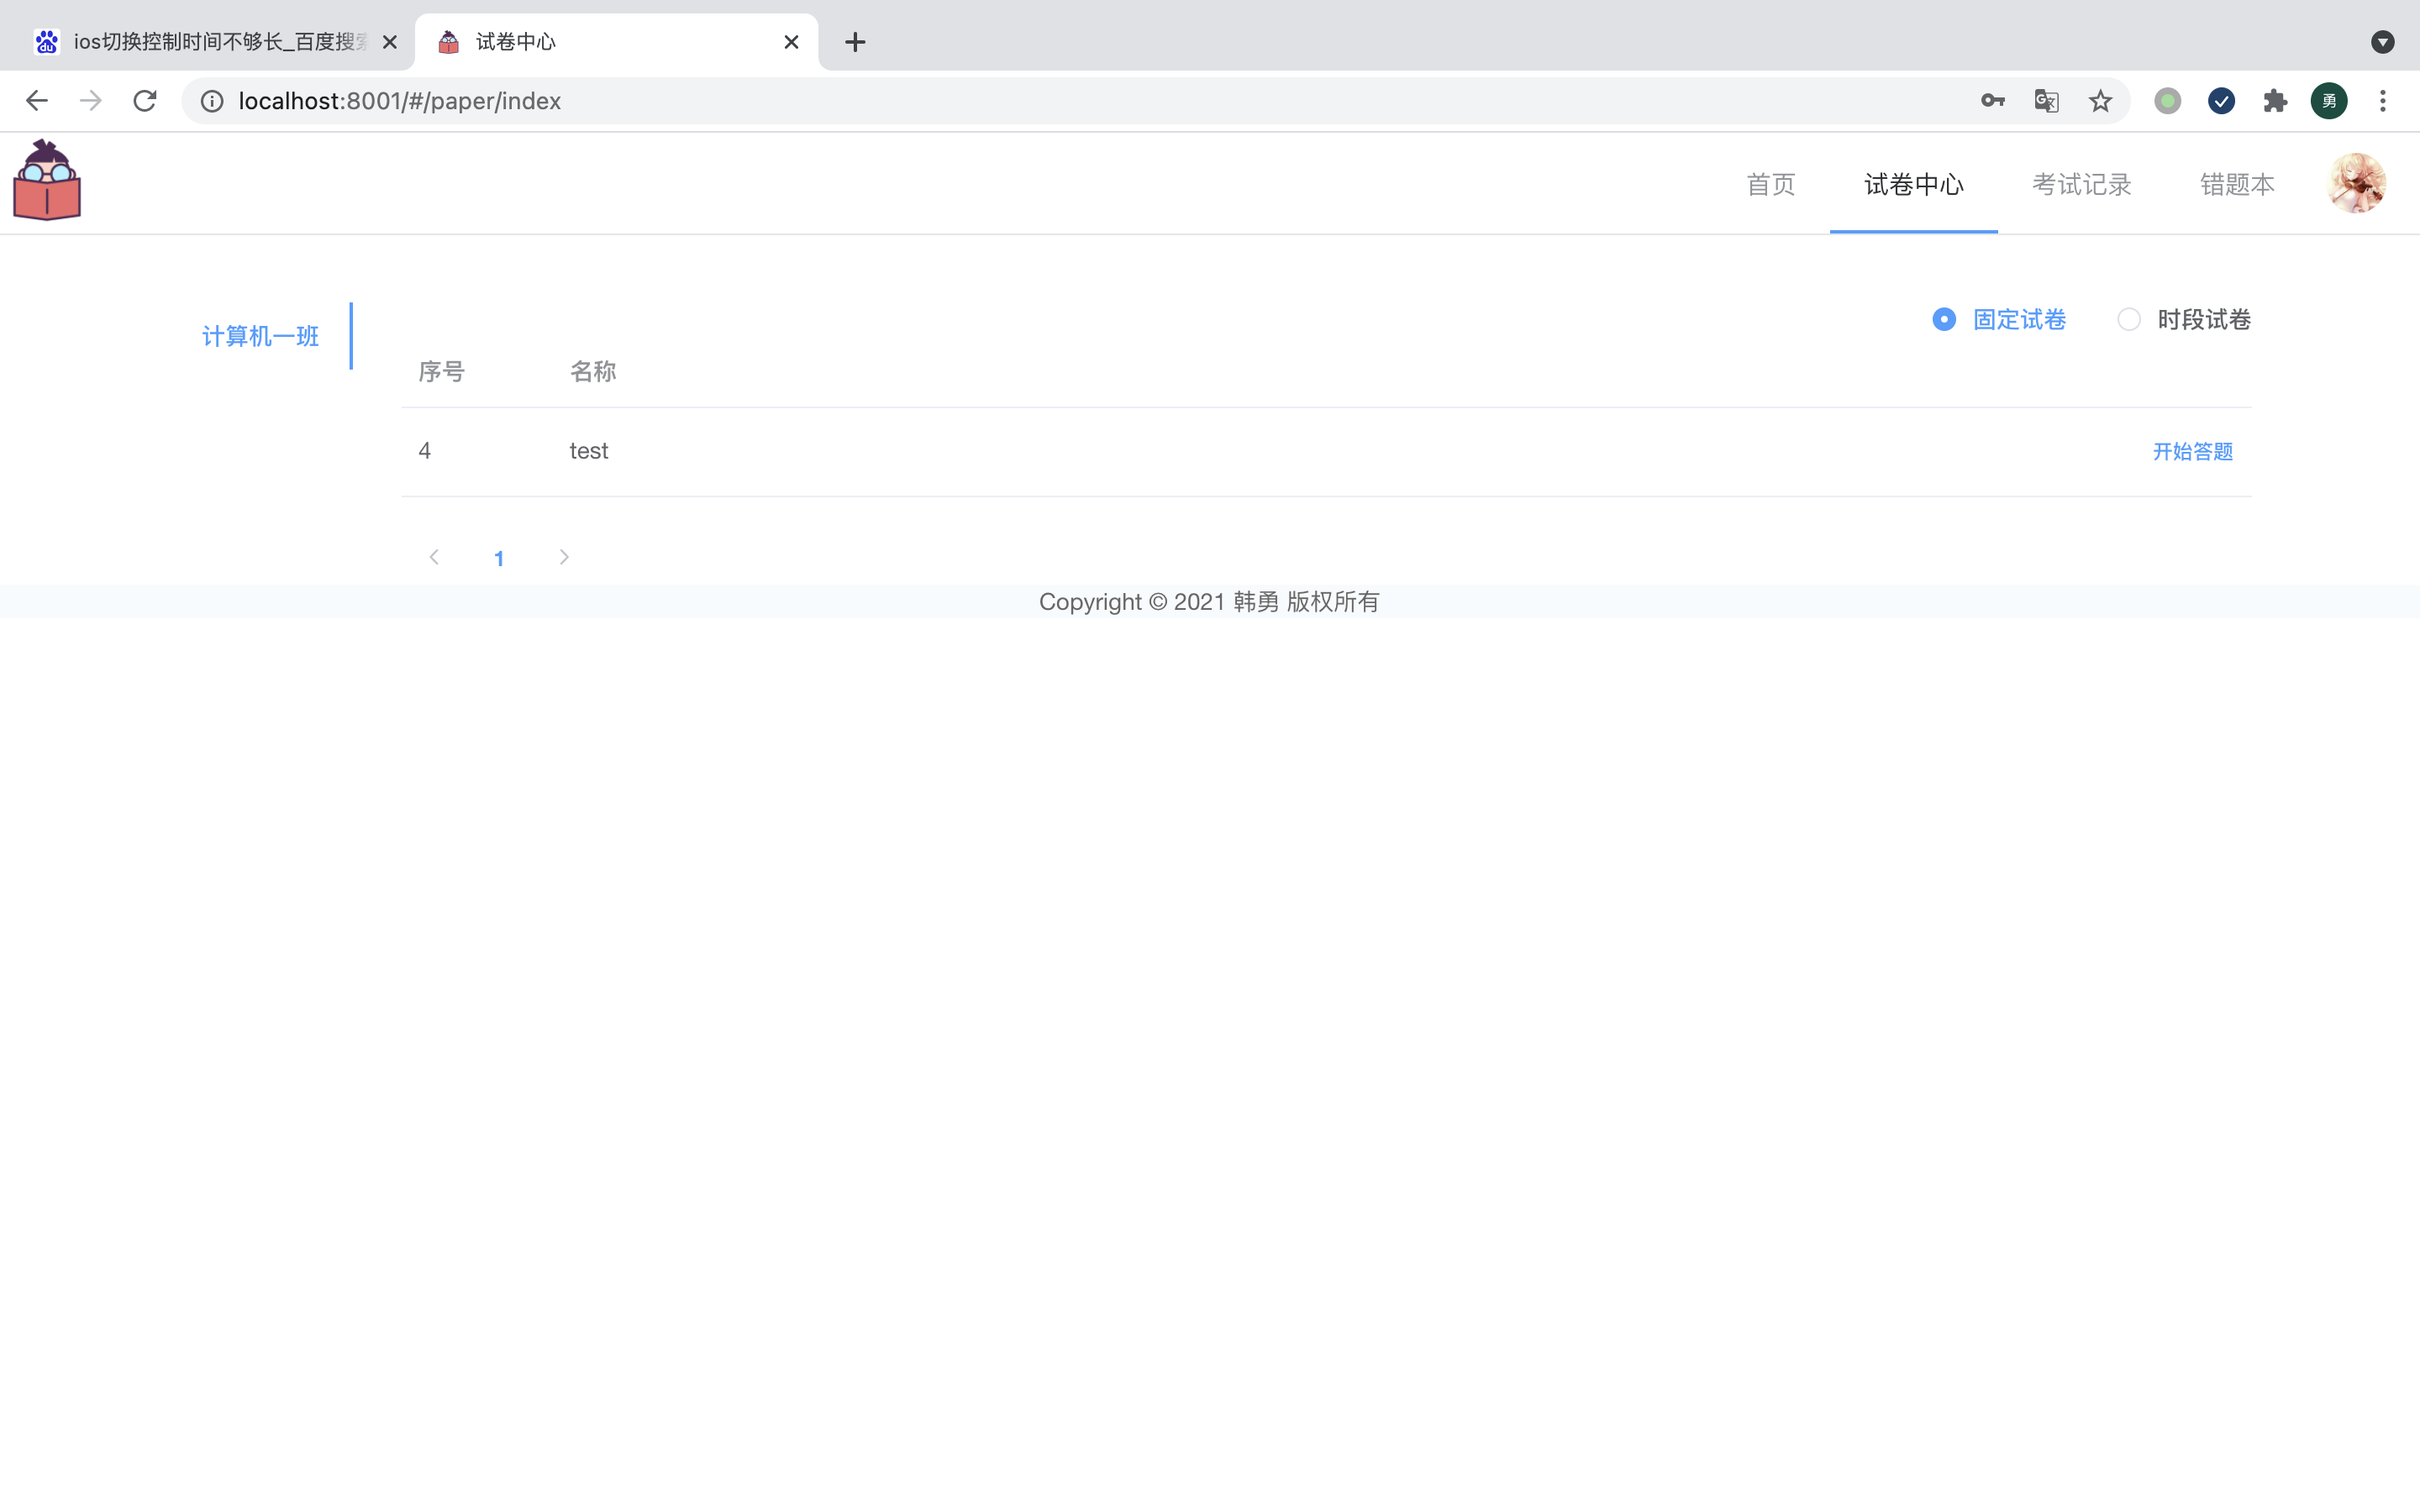
\includegraphics[width=1.0\textwidth,keepaspectratio]{data/chapter-5/student/shijuanzhongxin.png}
			\caption{学生试卷中心}
			\label{figure:szhongxin}
		\end{figure}
\end{enumerate}

\subsection{学生考试记录}
\begin{enumerate}
	\item[] \textbf{功能描述:}考试记录功能界面,学生可以通过该功能查看自己的考试记录和得分。
	\item[] \textbf{功能页面:}如图\ref{figure:sjilu}所示 \\
		\begin{figure}[H]
			\centering
			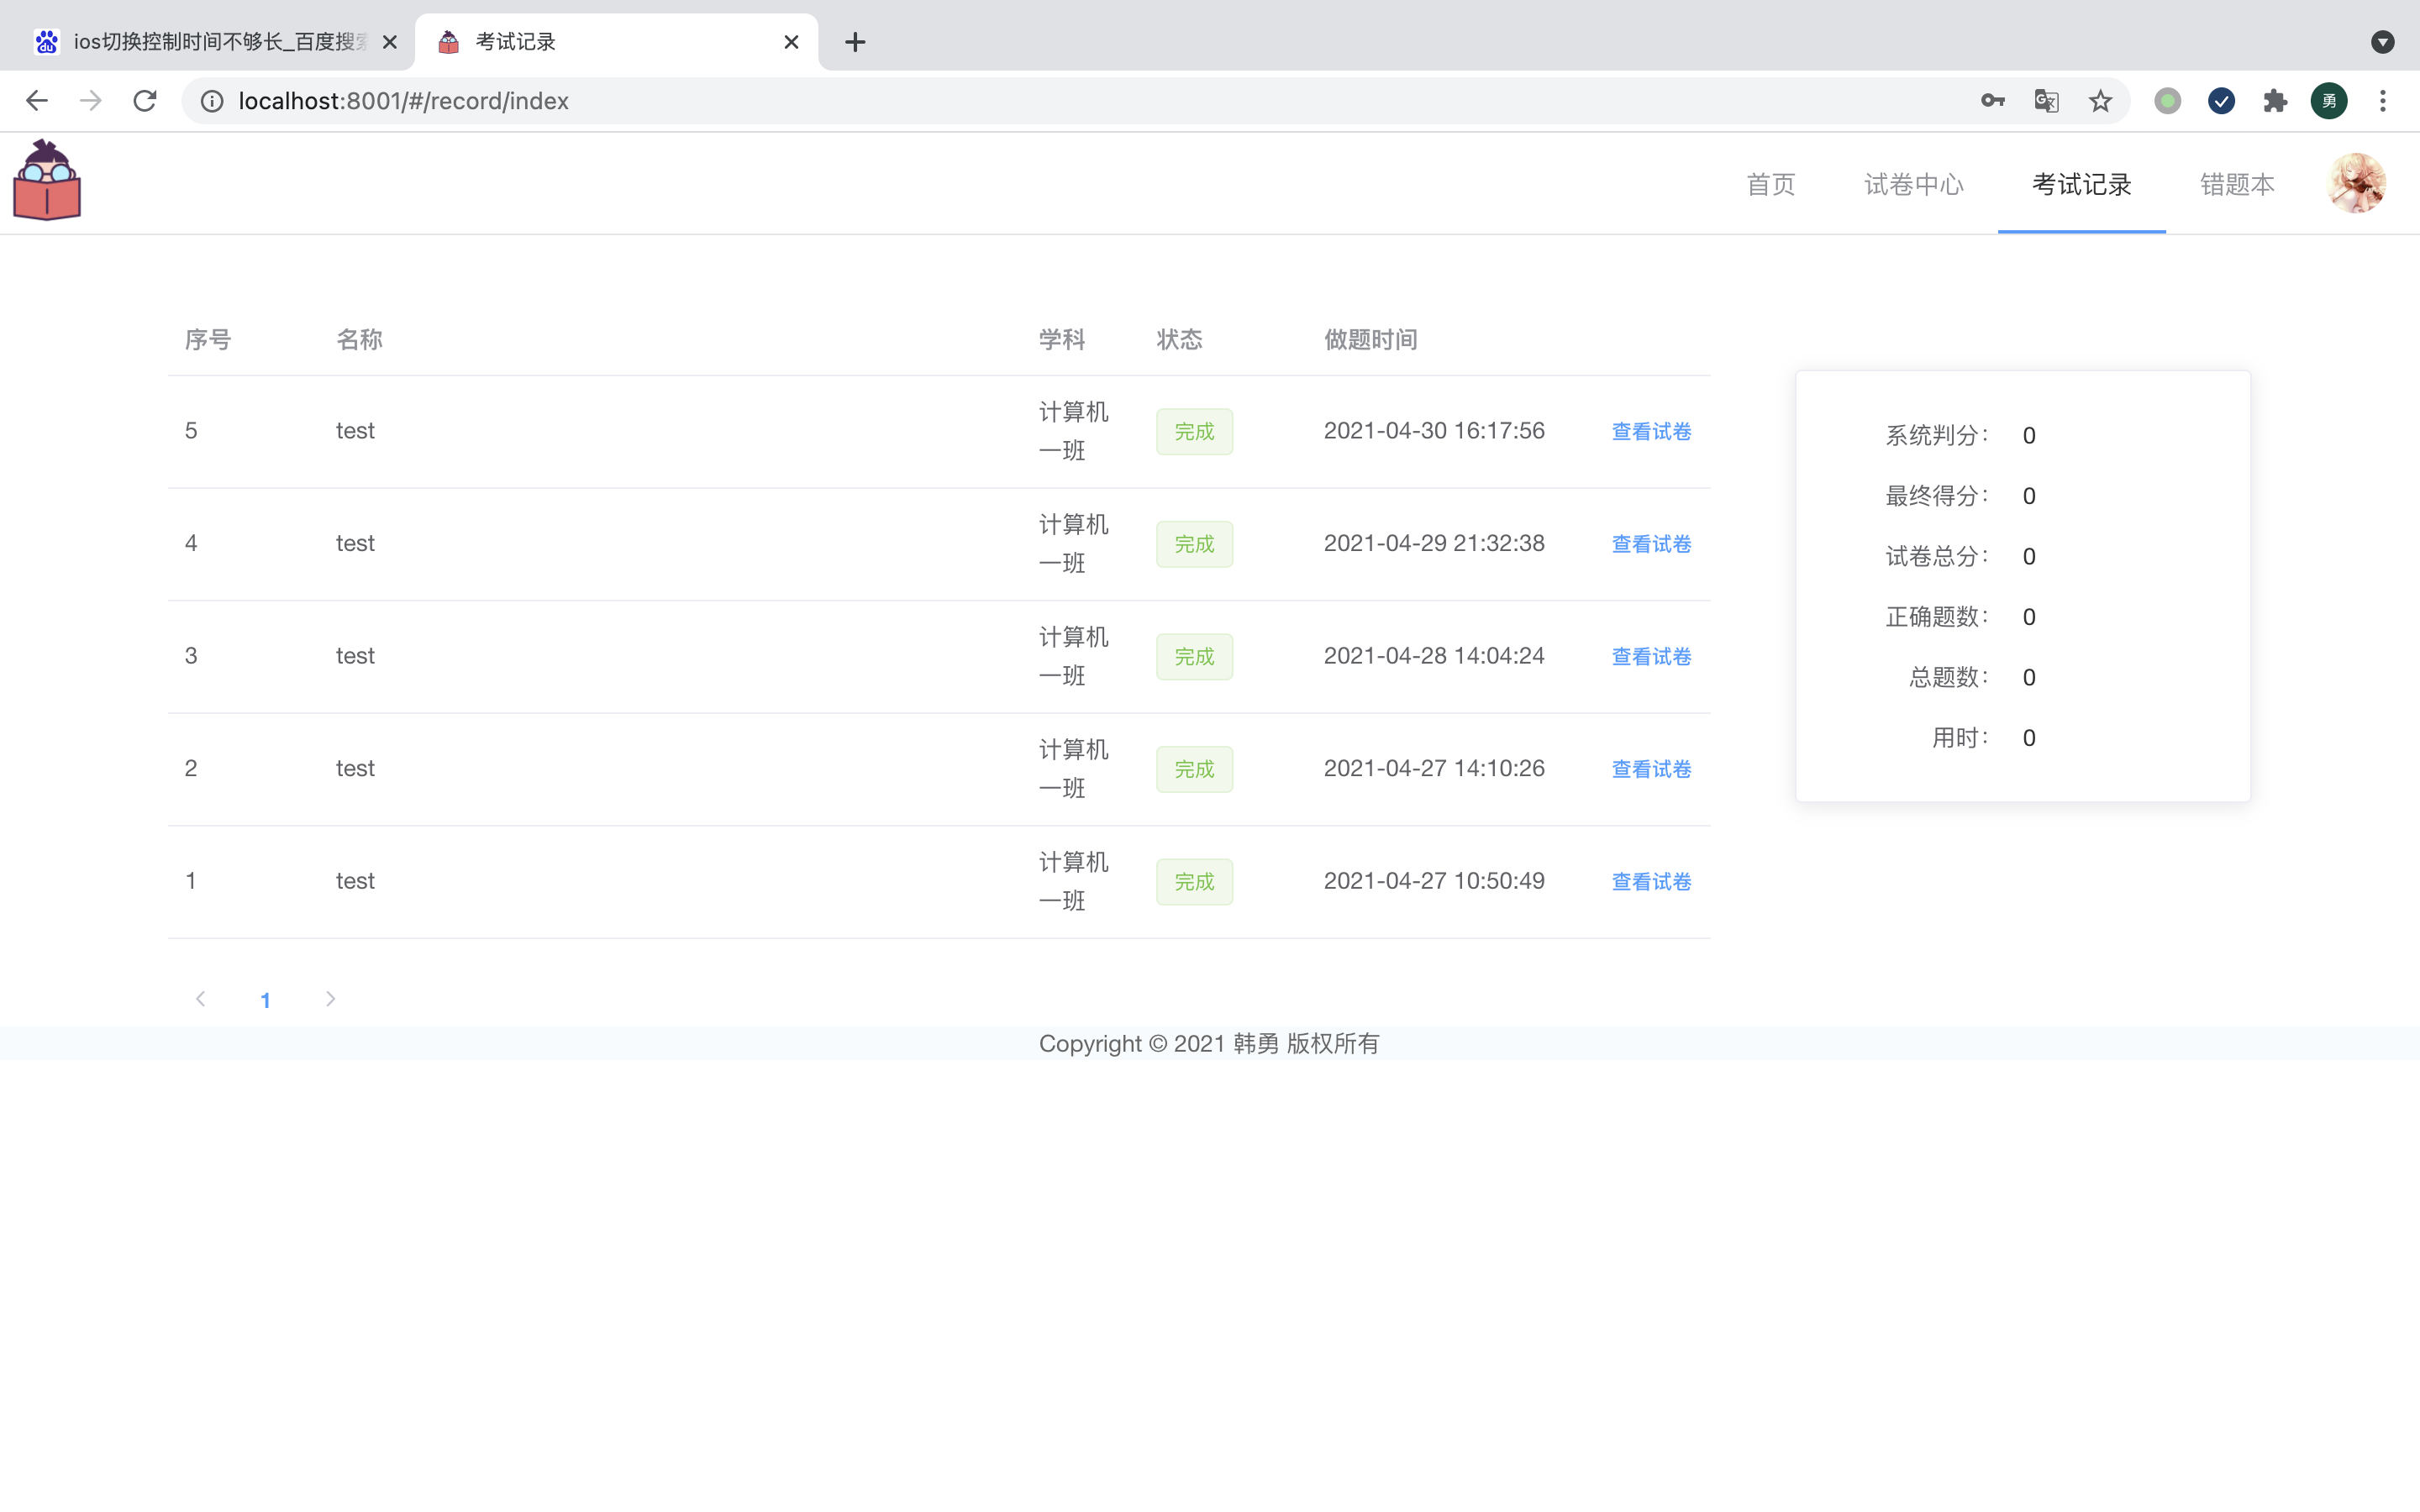
\includegraphics[width=1.0\textwidth,keepaspectratio]{data/chapter-5/student/kaoshijilu.png}
			\caption{学生考试记录}
			\label{figure:sjilu}
		\end{figure}
\end{enumerate}

\subsection{学生错题本}
\begin{enumerate}
	\item[] \textbf{功能描述:}错题本功能界面,学生可以通过该功能查看自己的历史错题,其中包括错误原因、正确答案和题目解析。
	\item[] \textbf{功能页面:}如图\ref{figure:scuotiben}所示 \\
		\begin{figure}[H]
			\centering
			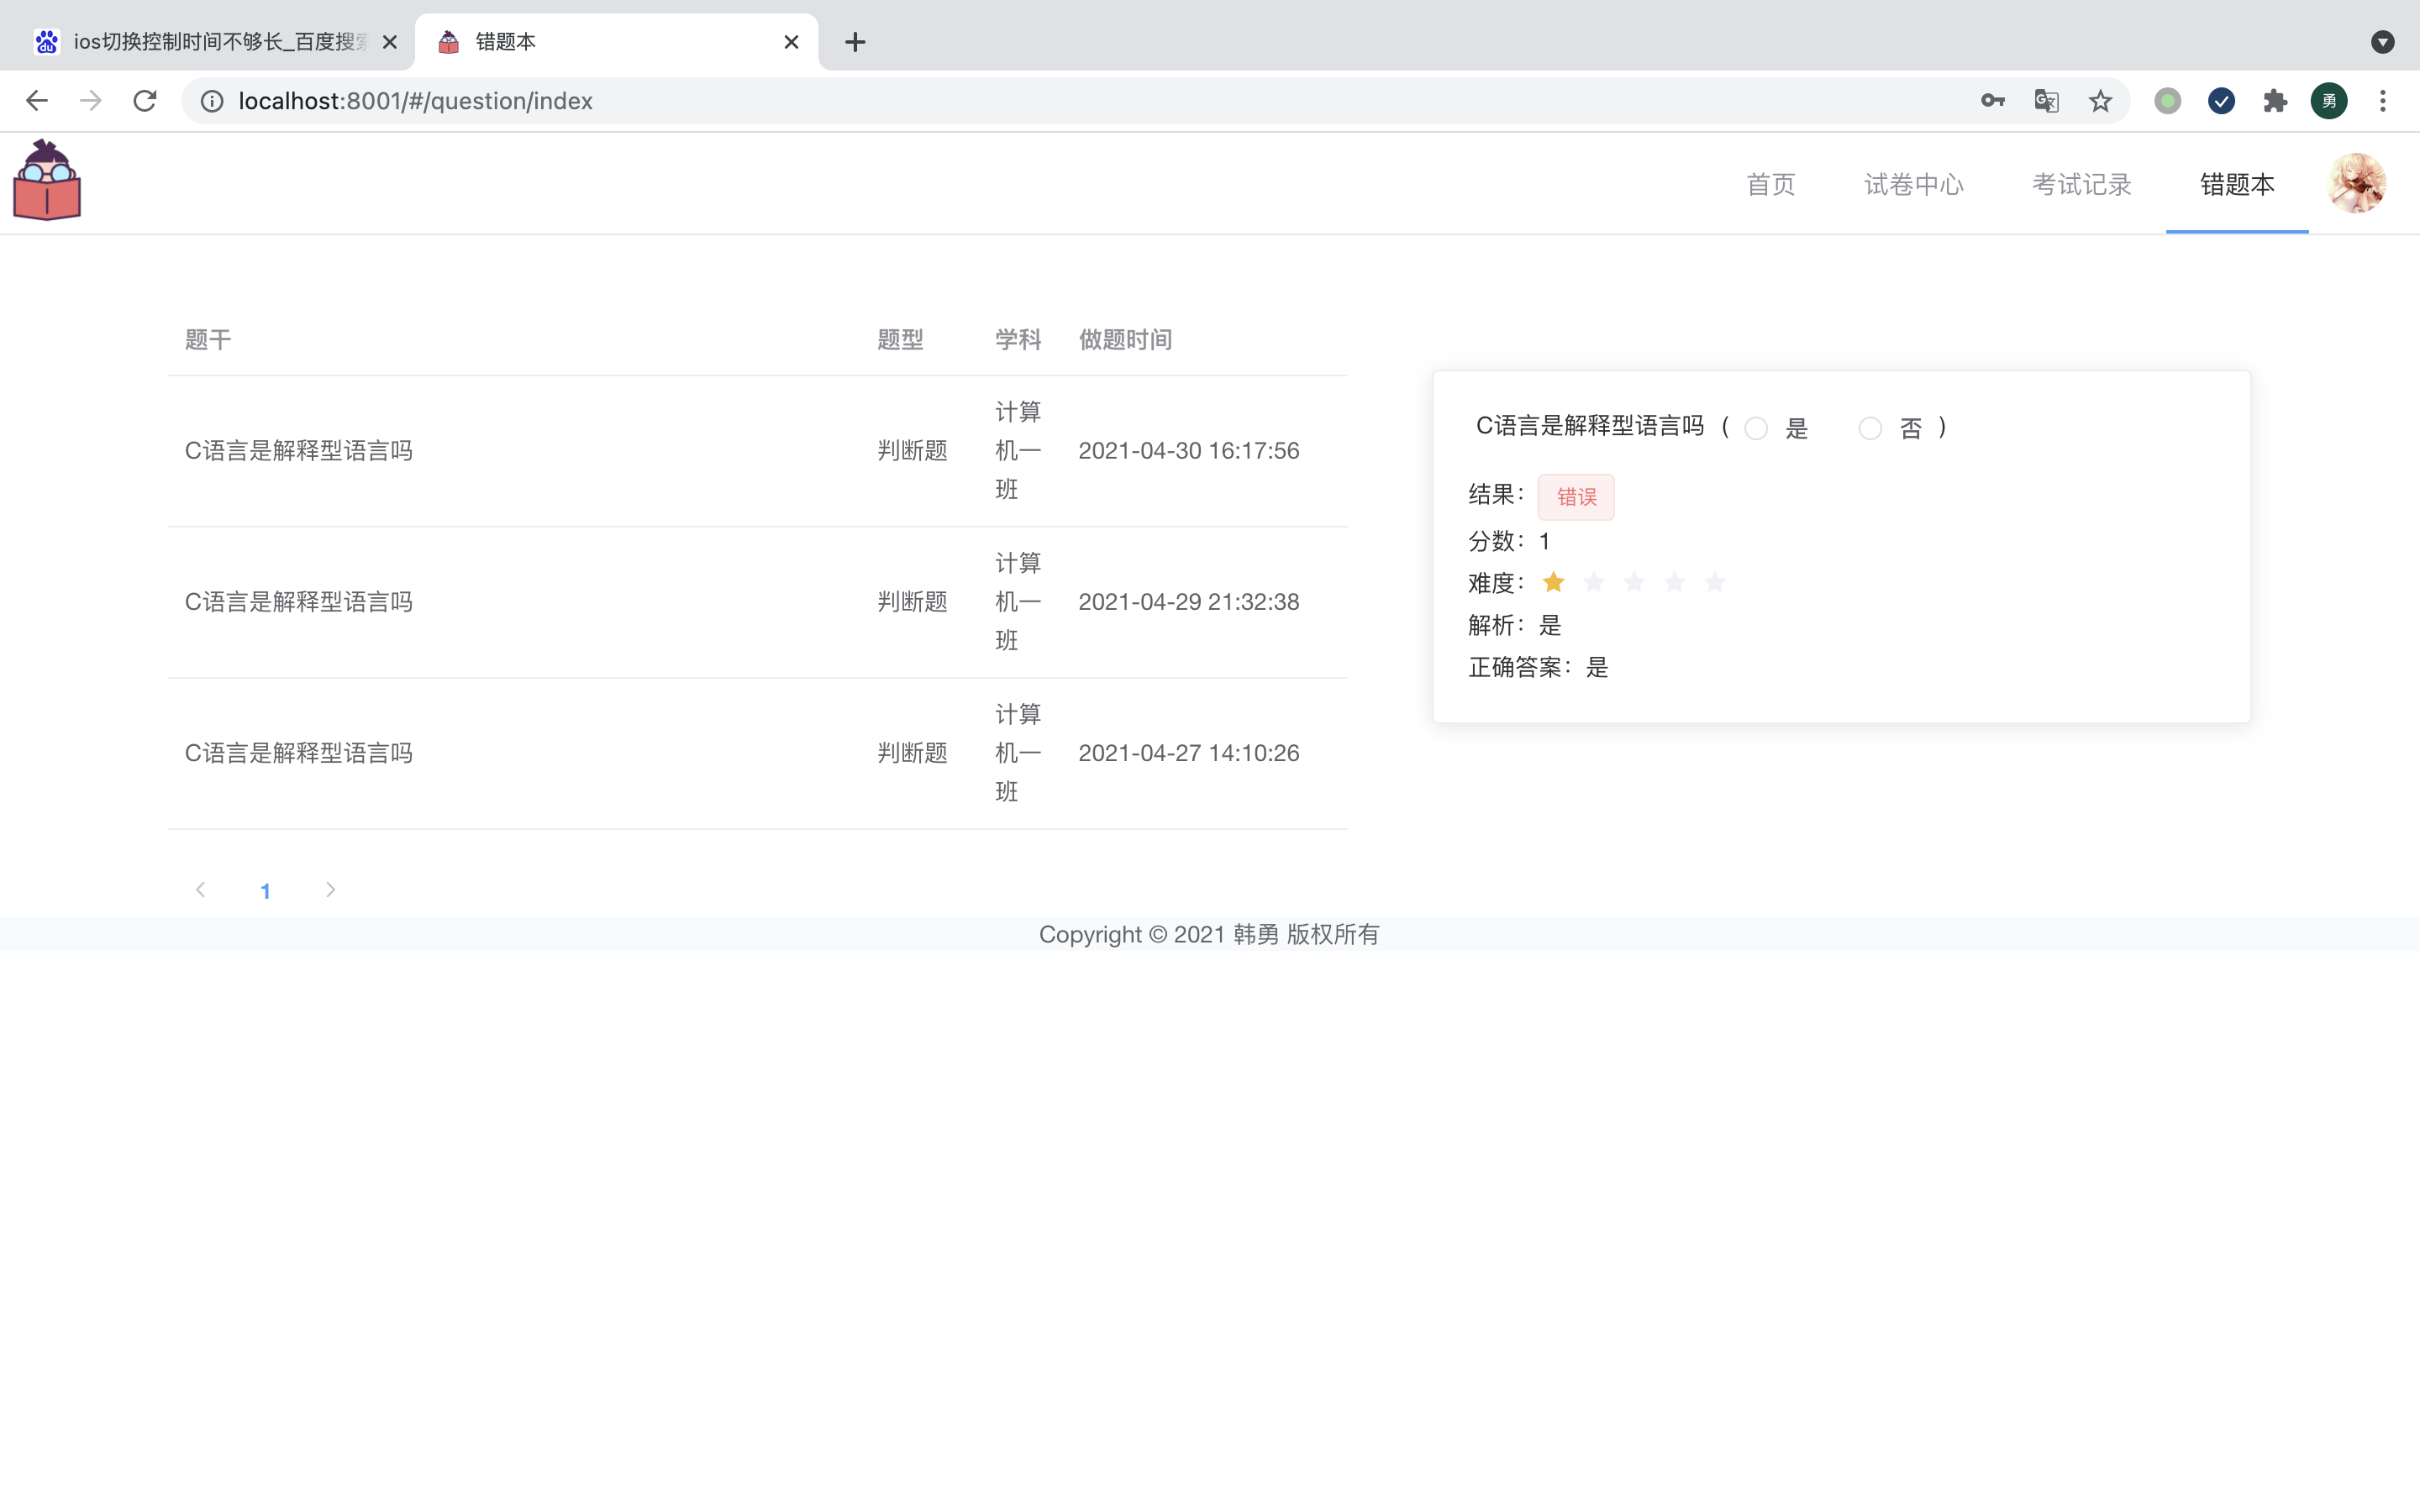
\includegraphics[width=1.0\textwidth,keepaspectratio]{data/chapter-5/student/cuotiben.png}
			\caption{学生错题本}
			\label{figure:scuotiben}
		\end{figure}
\end{enumerate}

\subsection{学生用户信息}
\begin{enumerate}
	\item[] \textbf{功能描述:}用户信息功能界面,学生可以通过该功能查看自己的个人信息并可以修改相关信息。
	\item[] \textbf{功能页面:}如图\ref{figure:sxinxi}所示 \\
		\begin{figure}[H]
			\centering
			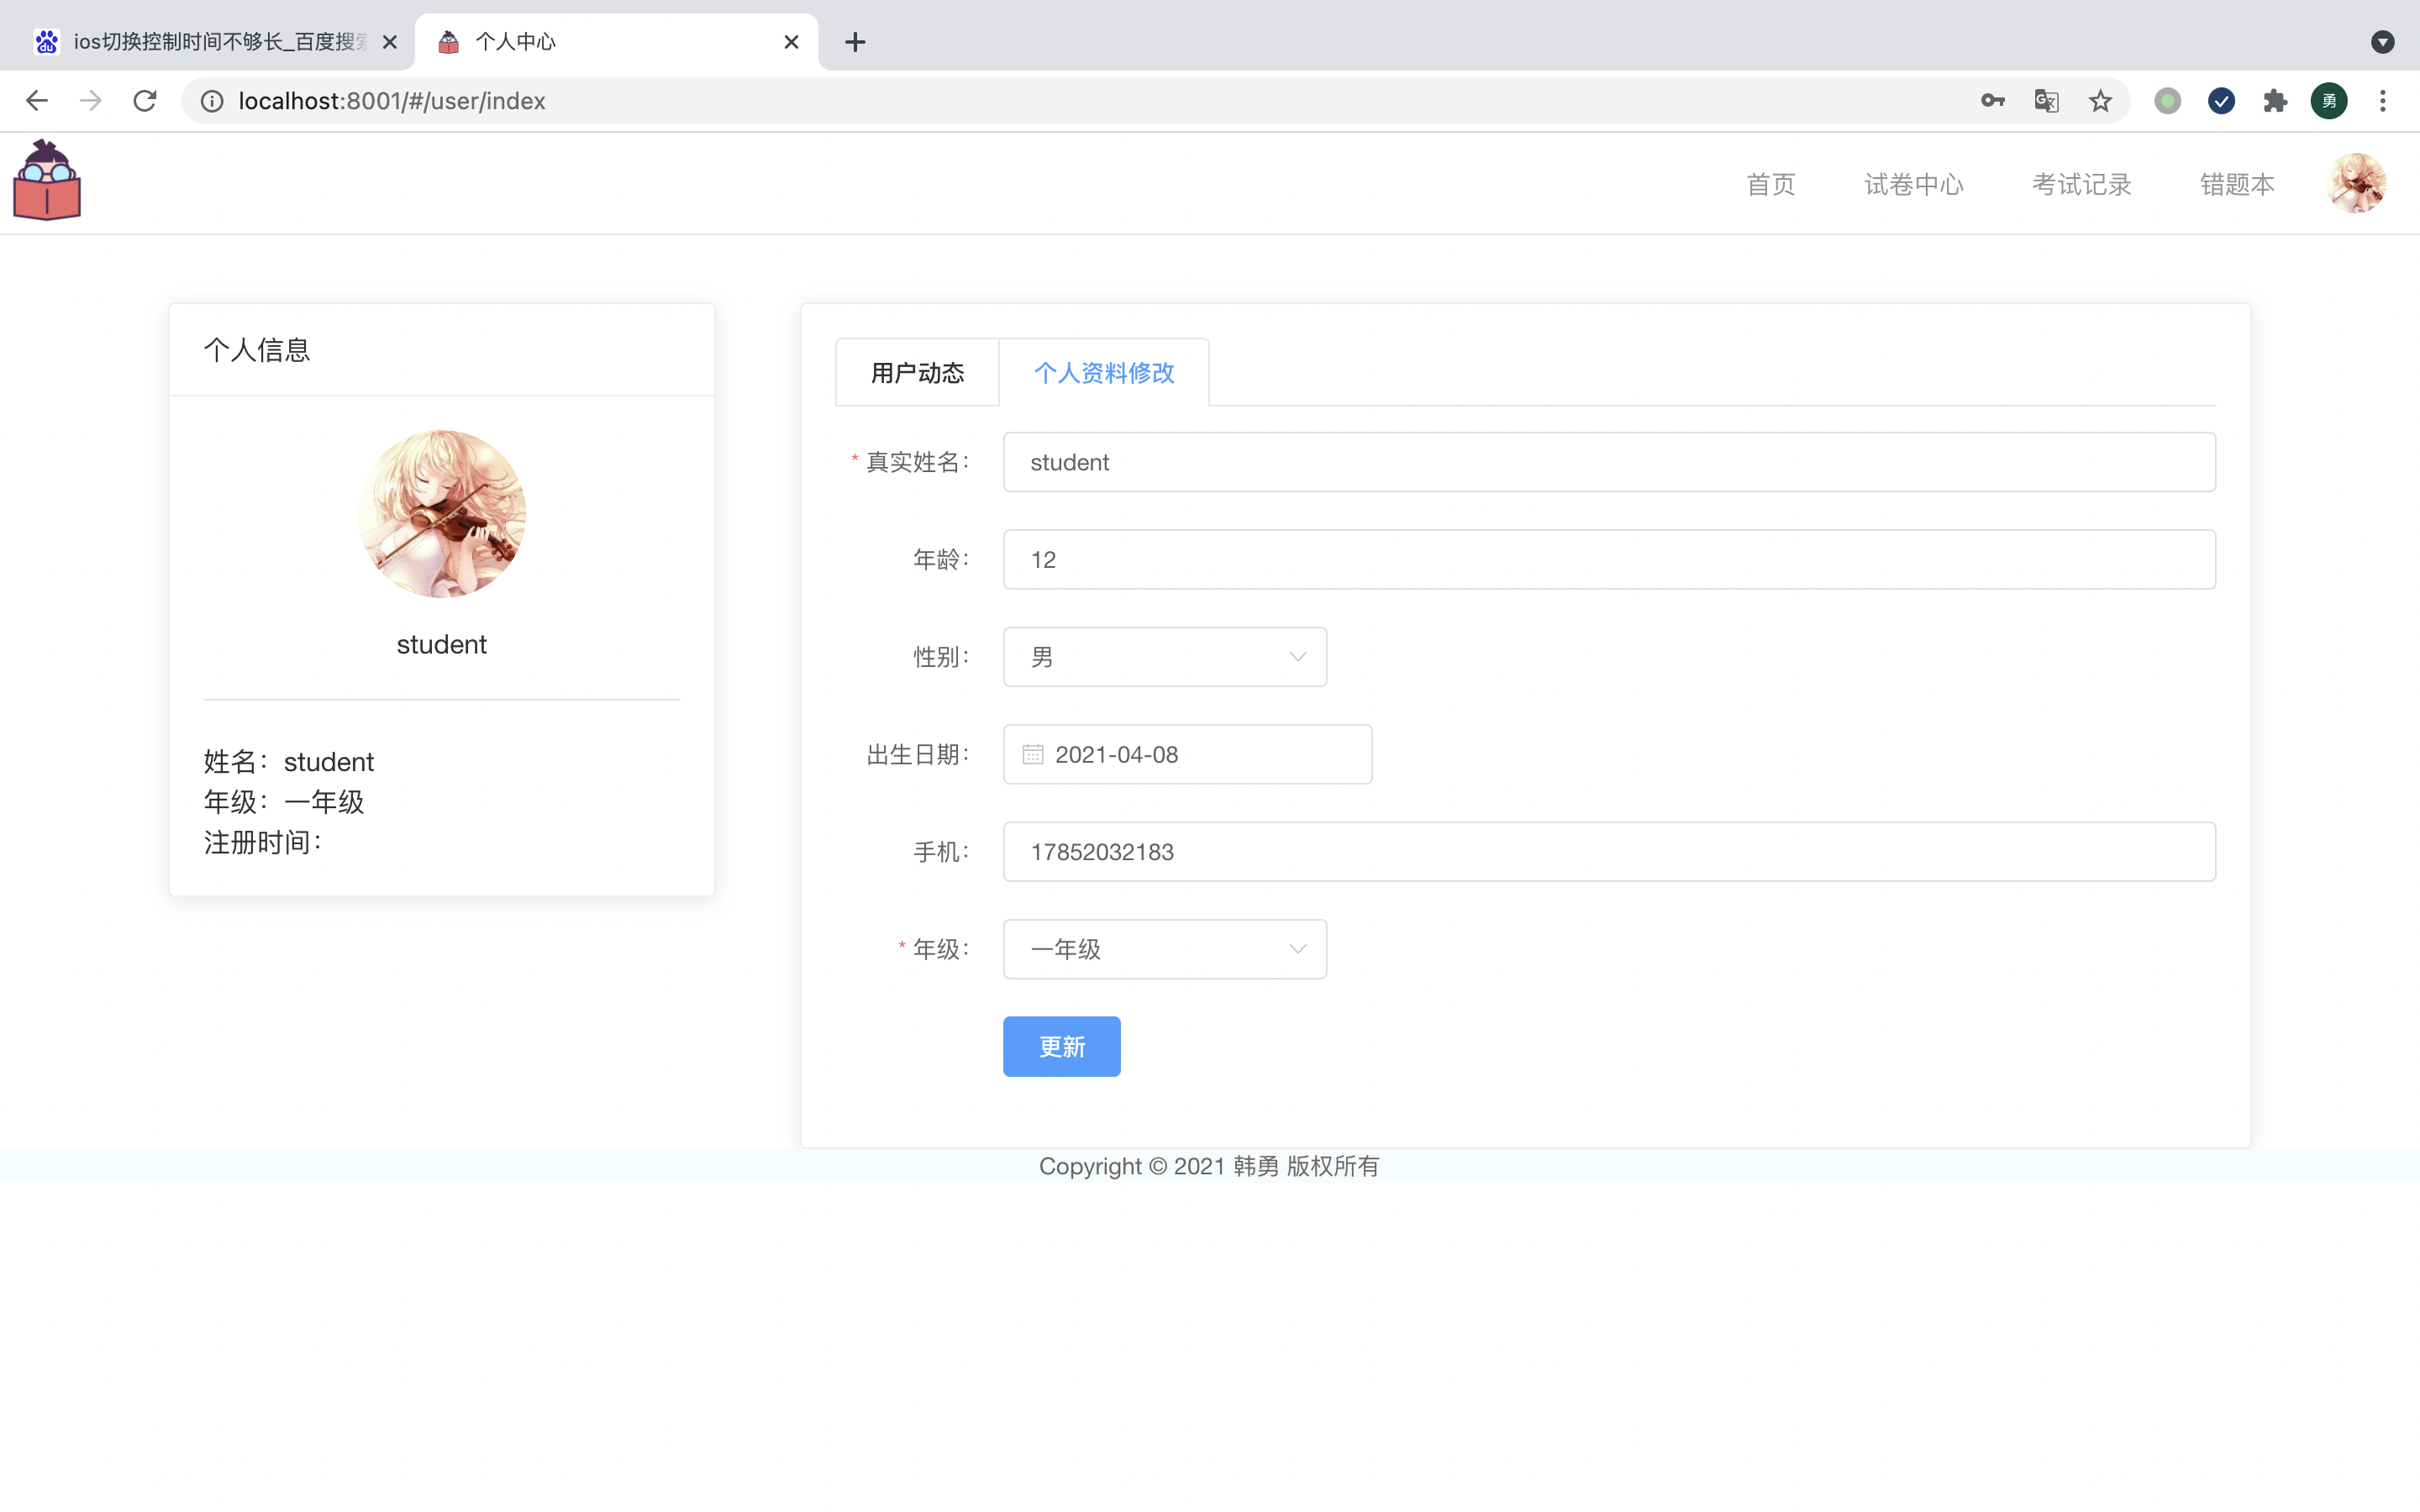
\includegraphics[width=1.0\textwidth,keepaspectratio]{data/chapter-5/student/yonghuxinxi.png}
			\caption{学生用户信息}
			\label{figure:sxinxi}
		\end{figure}
\end{enumerate}

\subsection{学生考试}
\begin{enumerate}
	\item[] \textbf{功能描述:}考试功能界面,学生开始考试或练习后会进入该界面,进入该页面后将自动开始录像并随机拍照对考试进行监控,考试时间结束后,考试将自动结束
	并提交,学生也可以在考试时间结束之前自行提交。
	\item[] \textbf{功能页面:}如图\ref{figure:skaoshi}所示 \\
		\begin{figure}[H]
			\centering
			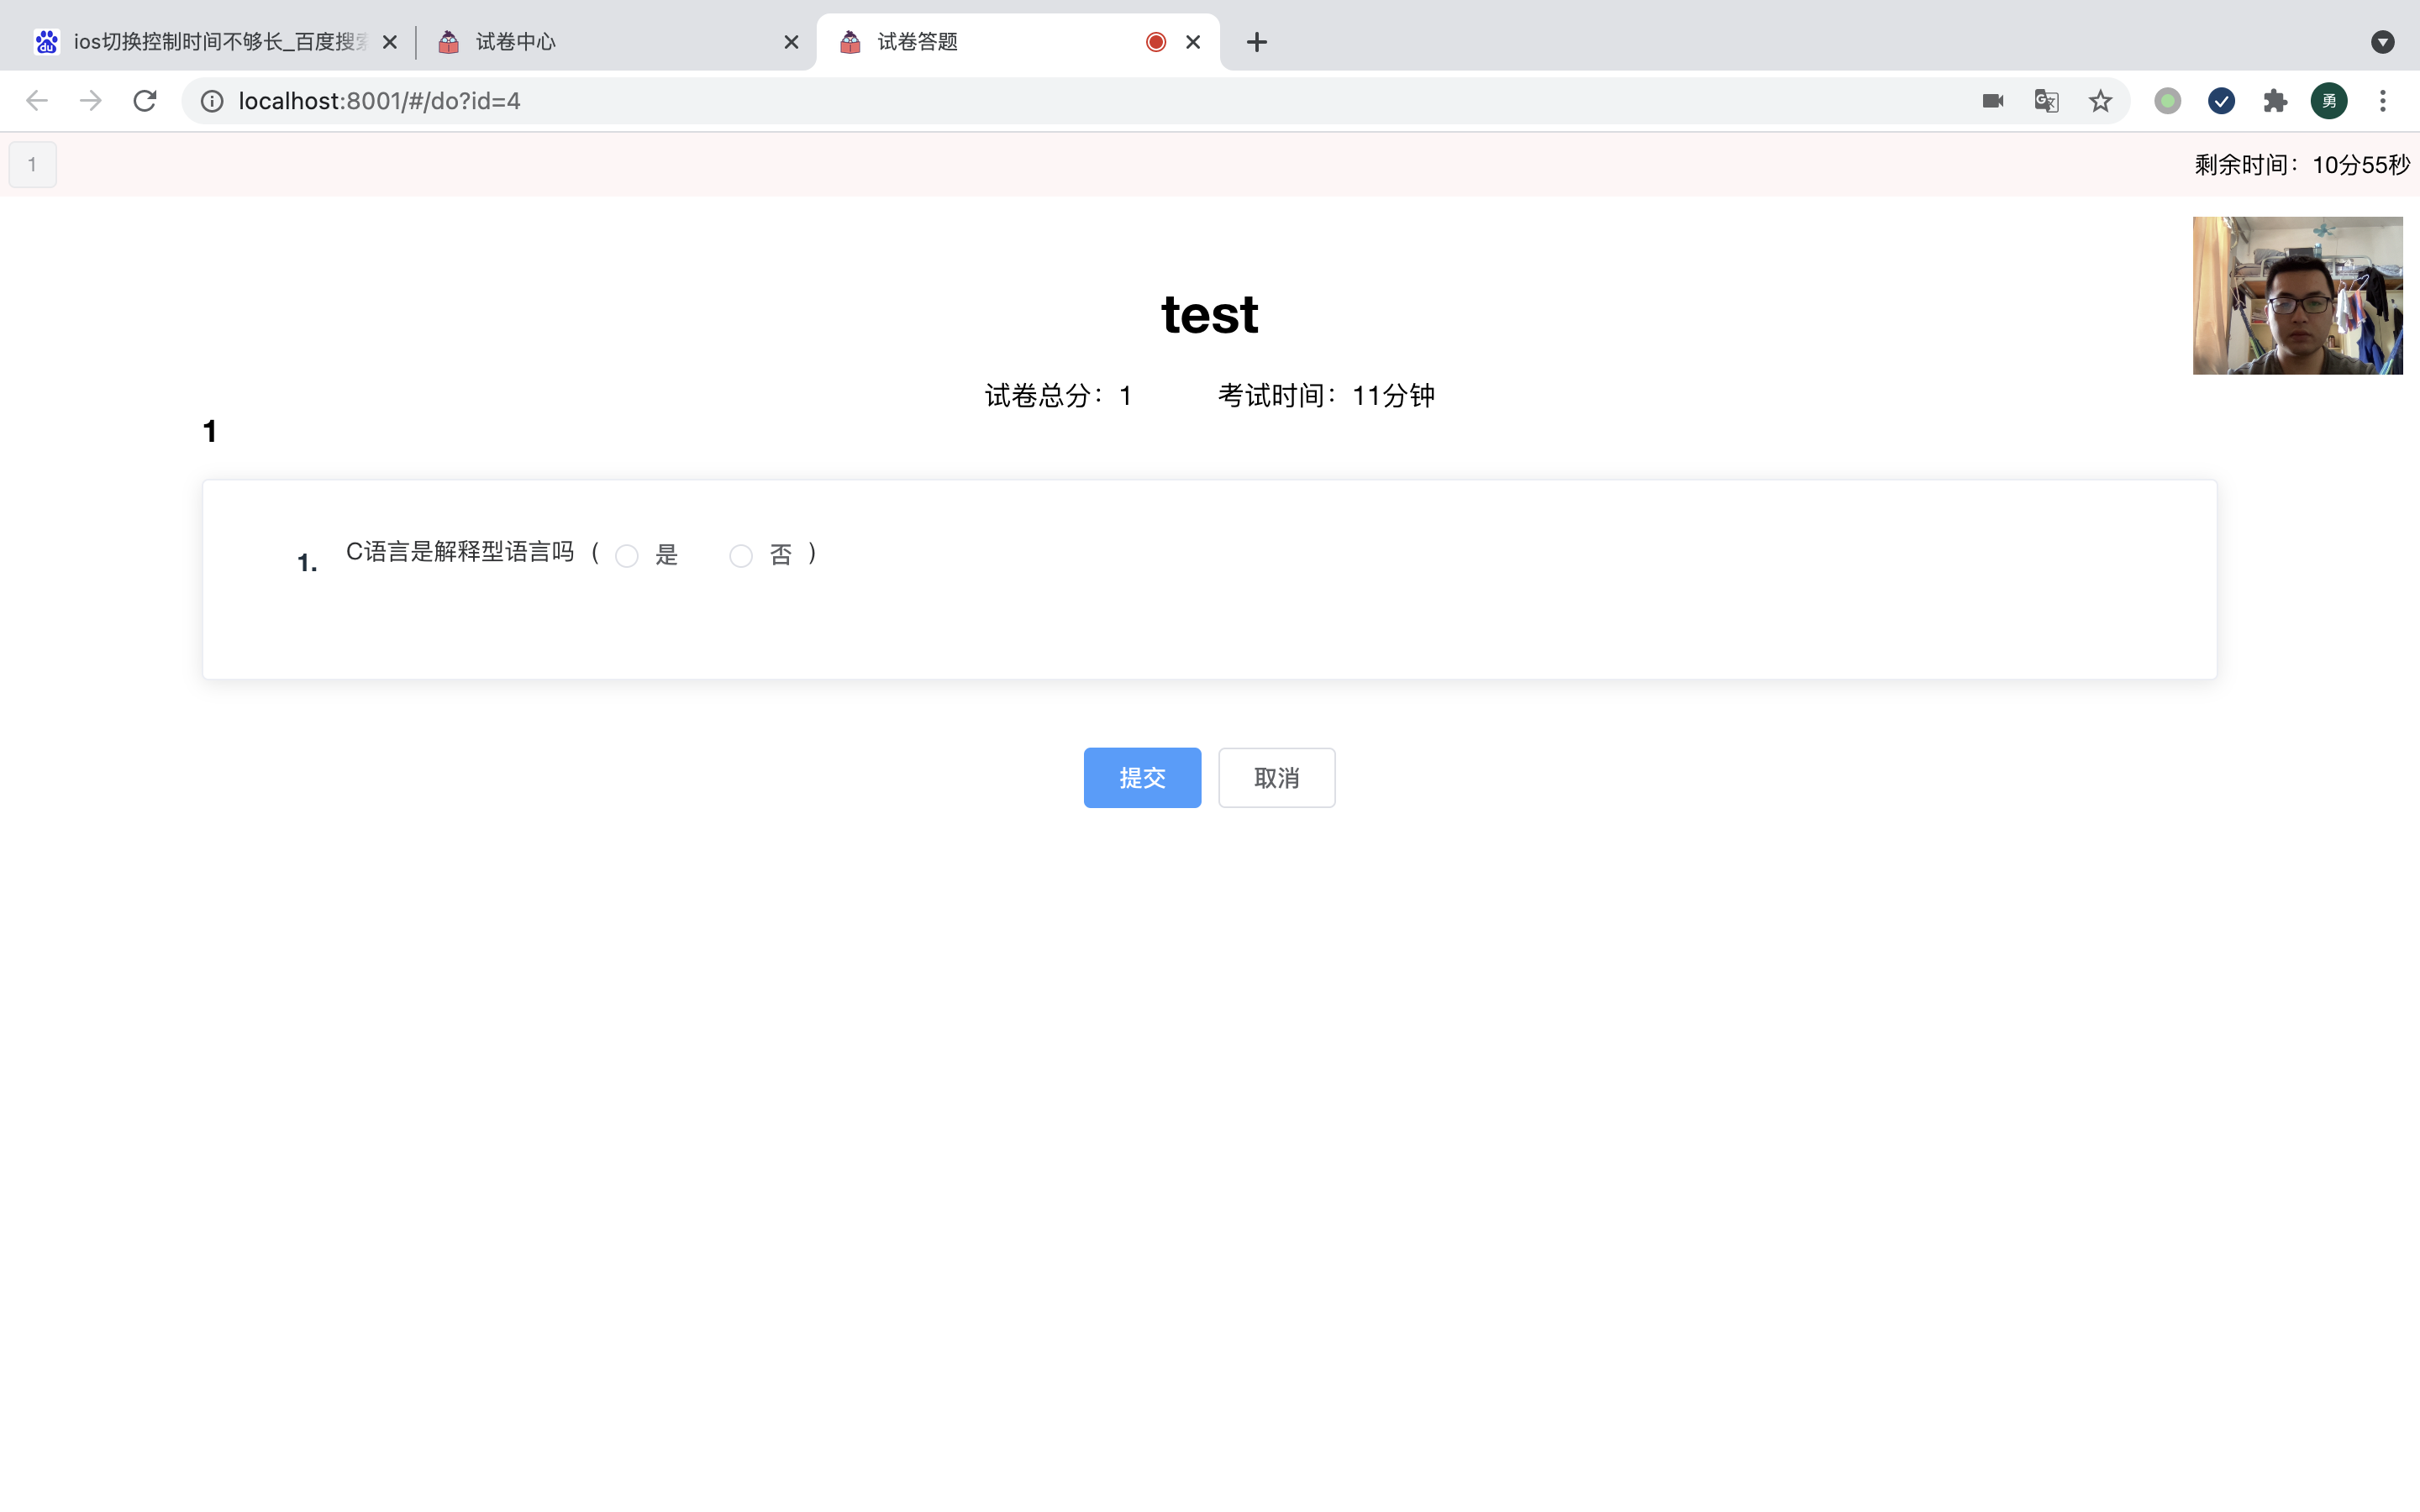
\includegraphics[width=1.0\textwidth,keepaspectratio]{data/chapter-5/student/kaoshi.png}
			\caption{学生考试}
			\label{figure:skaoshi}
		\end{figure}
\end{enumerate}